%
% CSML Final Project Paper
%

\documentclass[11pt,a4paper]{article}
\usepackage[hyperref]{acl2019}
\usepackage{times}
\usepackage{latexsym}
\usepackage{mathtools}
\usepackage{amsmath}
\usepackage{amsfonts}
\usepackage{amssymb}
\usepackage{float}
\usepackage{graphicx}
\usepackage{caption}
\usepackage{pgfplots}
\usepackage[inline]{enumitem} % note the [inline]
\pgfplotsset{compat=newest}
\usetikzlibrary{fit,backgrounds,positioning}
\usepackage{url}

\aclfinalcopy % Uncomment this line for the final submission

\newcommand\BibTeX{B\textsc{ib}\TeX}

\title{Yahtzee: Reinforcement Learning Techniques for Stochastic Combinatorial Games}

\author{Nick Pape \\
  nap626 \\
  \texttt{nickpape@utexas.edu} \\}

\date{2025-12-01}

\begin{document}
\maketitle
\begin{abstract}
  <ABSTRACT GOES HERE>
\end{abstract}

\section{Introduction}
% <600-900 words>
% 342 words
\subsection{Yahtzee as a Reinforcement Learning Benchmark}
While on the surface \textit{Yahtzee} appears to be a trivial dice game \cite{hasbro-2022-yahtzee-rules}, it is actually a complex stochastic optimization problem with combinatorial complexity.

Although there are methods for computing optimal play in \textit{Yahtzee} using dynamic programming, these are computationally expensive and do not scale well to multiplayer settings.
\textit{Yahtzee} offers a rich environment for testing reinforcement learning (RL) solutions due to its combination of a large but manageable state space, randomness, ease of simulation, subtle strategic considerations, and easily identifiable subproblems.
While there have been a small number of efforts to create RL agents for \textit{Yahtzee}, a comprehensive approach using self-play has yet to be published.
It remains an open question of whether deep RL methods can approach optimal performance in full-game \textit{Yahtzee}, and which architectural and training choices most affect learning efficiency and final performance.
Similarly, a robust RL-based solution for multiplayer \textit{Yahtzee} using RL methods has yet to be demonstrated.

\textit{Yahtzee} is an ideal candidate to serve as a bridge between simple toy problems such as \textit{Lunar Lander} \cite{brockman2016openai} and extremely complex games like Go \cite{silver2016alphago}.
Typical small benchmarks often offer low stochasticity and simple combinatorics whereas complex games have intractable state spaces and require massive computational resources and heavy engineering to solve.
\textit{Yahtzee} sits in a middle ground where an analytic optimum exists, but reaching it with RL methods is non-trivial.
These factors make it a challenging yet feasible benchmark for RL research.

\subsection{Objectives}

In this paper we aim to methodically study whether a deep RL agent can achieve near DP-optimal performance in full-game solitaire \textit{Yahtzee} using only self-play,
and how architectural and training choices affect learning efficiency.

Concretely, we ask: \begin{enumerate*}[label=(\roman*)]
  \item How does the trade-off between maximizing single-turn expected score and full-game performance behave?
  \item Can an agent reach optimal performance under a fixed training budget, using only self-play?
  \item Which design choices (state and action encodings, credit assignment, variance controls, baselines, entropy, etc) most affect final performance?
  \item What failure modes exist in learned policies and how can they be addressed?
  \item Can we find a successful architecture which could be adapted to multiplayer \textit{Yahtzee}?
\end{enumerate*}

\section{Related Work}
% <600-800 words>
% 1097 words

\subsection{Policy Gradient Methods and Variance Reduction}
\subsubsection{Return Estimation}
In this paper, we follow notation from \citet{sutton-2018-reinforcement-book} and the policy gradient theorem \cite{sutton-2000-policy-gradient}.

In long episodic games, the choice of return calculation affects sample efficiency, bias, and variance.
Monte-Carlo (MC) returns $G_{t}^{MC}$ use a summation over the full series of rewards until the end of the episode.
This approach is unbiased but has high variance.
In contrast, Temporal Difference methods use a "bootstrapped" estimate of future rewards to reduce variance.
Essentially, they only consider received rewards $R$ in a specific time window, and use an estimate from the value function $V(S_{t+1})$ for future rewards beyond that window; this is called the TD estimate \cite{sutton-2018-reinforcement-book}.

This time window can also be adjusted, depending on the task.
For example, n-step returns $G_{t}^{TD(n)}$  interpolate between MC and single-step TD returns, allowing us to define a time horizon $n$ over which to sum rewards before bootstrapping.
This lets us manually control the bias-variance tradeoff.
A related method is $TD(\lambda)$, which uses an exponentially weighted average of n-step returns, effectively blending multiple time horizons into a single estimate controlled by $\lambda$ \cite{sutton-2018-reinforcement-book}.

While TD estimates are biased (since they rely on future value estimates to be accurate), they have much lower variance than full-episode returns.
In TD(0), the value function effectively learns using a single timestep; this is a much simpler problem than estimating the entire sequence of rewards.
This often makes TD methods more sample efficient than REINFORCE, and provides the benefit of being able to learn online rather than waiting until the end of an episode.

Pure TD methods can also be viewed as a form of approximate dynamic programming, making them a natural fit for domains where dynamic-programming solutions exist \cite{bertsekas1996neuro}.

\subsubsection{Policy Gradient Methods}
Policy-gradient methods are a family of algorithms which directly optimize a parameterized policy $\pi_{\theta}$ to follow an estimate of the performance gradient.
A simple formulation of this is the REINFORCE algorithm \cite{williams-1992-reinforce}, which uses Monte-Carlo returns $G_{t}^{MC}$ on finite, episodic tasks; however, while unbiased, it suffers from high variance.
One trick for reducing variance in REINFORCE is to subtract a baseline (often just an average return, but potentially a learned estimate) from an episode's MC return.
This yields an advantage estimate that reduces variance without changing its expectation \cite{weaver2013optimal, greensmith-2004-variance-reduction}.

Actor-critic methods \cite{konda-1999-actorcritic} such as Advantage Actor-Critic (A2C) and Asynchronous Advantage Actor-Critic (A3C) \cite{mnih-2016-a3c} typically use a TD-style return estimate to update the policy.
These methods learn a separate value function: the critic $V_{\phi}$.
This critic is used directly in the TD return estimate as the bootstrap value estimate for a state.
For these methods, we can define the TD error $\delta_t$ as the difference between the TD estimate and the value estimate for the current state $V(S_t)$.
This $\delta_t$ error is then used as the advantage estimate for a normal policy gradient update \cite{konda-1999-actorcritic}.

Another widely used algorithm, proximal policy optimization (PPO), utilizes a clipped objective $L^{CLIP}(\theta)$
and explicit Kullback-Leibler (KL) divergence control to dramatically reduce variance and ensure stable updates \cite{schulman-2017-ppo}.
PPO uses the Generalized Advantage Estimate (GAE), which is closely related to $TD(\lambda)$, applying a $\lambda$-weighted mixture at the level of advantages \cite{schulman-2016-gae}.

\subsubsection{Other Variance Reduction Techniques}
Aside from return estimation, there is a host of other variance reduction techniques which can be employed for policy gradient methods.

Normalizing advantages across a batch improves gradient conditioning and is common practice \cite{schulman2015trpo}.
Entropy regularization prevents early collapse to suboptimal policies by encouraging exploration via the addition of an explicit entropy bonus term in the loss function \cite{williams-peng-1991-function-optimization, mnih-2016-a3c, schulman-2017-ppo}.
Gradient clipping is frequently used alongside these techniques to stop rare, but large, gradient updates from destabilizing training \cite{pascanu-2013-rnn-clipping}.
While high variance is unavoidable in deep reinforcement learning, poor performance can often be linked to numerical instability rather than inherent flaws in algorithmic design \cite{bjorck-2022-high-variance};
simple tweaks like normalizing features before activations can dramatically improve stability.

\subsubsection{Reward Shaping}
<Do we need a section on reward shaping?>

\subsection{Complex Games}
Typical board and dice games have extreme state complexity or stochasticity; reinforcement learning methods are a natural fit for these problems.
In a classic example, \citet{tesauro1995tdgammon} utilized temporal difference learning to achieve superhuman performance in \textit{Backgammon}, another game with a large state space and stochastic elements.
Tetris, which is deterministic but combinatorial, has also been studied extensively; \citet{bertsekas1996tetris} utilized approximate dynamic programming methods to learn effective policies for the game,
while \citet{gabillon2013tetris} effectively tackled the game using reinforcement learning methods.
\citet{moravcik2017deepstack} demonstrated that \textit{Texas Hold'em}, a stochastic game with hidden information, could be effectively learned.
Many other stochastic games can be learned well, so long as methods which ensure better exploration are used \cite{osband2016bootstrappeddqn}.
Lastly, RL methods can be used to reach superhuman performance on adversarial games, even despite their sparse reward structures.
For example, the game of Go, which has a notoriously intractable state space was solved using Monte-Carlo Tree Search and deep value networks \cite{silver2016alphago}.
Subsequent work showed Go could be learned without the use of expert data, purely through self-play \cite{silver2017alphagozero}.
In total, these works establish that RL methods can handle highly stochastic, combinatorial games, suggesting that \textit{Yahtzee} is a natural but underexplored candidate in this family.

\subsection{DP Methods for Yahtzee}
Solitaire \textit{Yahtzee} is a complex game with an upper bound of $~7 \times 10^{15}$ possible states in its state space.
It has a high degree of stochasticity, as dice rolls are the primary driver of state transitions.
Despite this, it has been analytically solved using dynamic programming techniques; \citet{verhoeff-1999-solitaire-yahtzee}, calculated that the average score achieved during ideal play is $254.59$ points, which serves as the gold-standard baselline for solitaire \textit{Yahtzee}.
Later work by \citet{glenn-2006-optimal-yahtzee} optimized the DP approach via symmetries to propose a more efficient algorithm for computing the optimal policy, with a reachable state space of $~5.3 \times 10^8$ states \cite{glenn-2007-solitaire-yahtzee}.

However, adversarial \textit{Yahtzee} remains an open problem.
While \citet{pawlewicz-2011-multiplayer-yahtzee} showed that DP techniques can be expanded to 2-player adversarial \textit{Yahtzee}, they do not scale to more players due to the exponential growth of the state space.
Approximation methods must be utilized for larger player counts.

\subsection{Reinforcement Learning for Yahtzee}
Some prior attempts have been made to apply reinforcement learning to \textit{Yahtzee}.
YAMS attempted to use Q-learning and SARSA to attempt to learn \textit{Yahtzee}, but was not able to surpass $~120$ points median \cite{belaich-2024-yams}.
Likewise, \citet{kang-2018-yahtzee-rl} applied hierarchical MAX-Q, achieving an average score of $129.58$ and a 67\% win-rate over a 1-turn expectimax agent baseline.
\citet{vasseur-2019-strategy-ladders} explored strategy ladders for multiplayer \textit{Yahtzee}, to understand how sensitive Deep-Q networks were to the upper-bonus threshold.
Later, \cite{yuan-2023-two-player-yahtzee} applied Deep-Q networks to the adversarial setting, with moderate success.

Additionally, some recent informal work has reported success using RL methods for \textit{Yahtzee}.
For example, Yahtzotron used heavy supervised pretraining and A2C to achieve an average of $~236$ points \cite{Haefner2021Yahtzotron}.
Although not a true reinforcement learning approach, \citet{DutschkeYahtzee} reports a statistical agent achieving a score of $241.6 \pm 40.7$ after just 8,000 games, using a combination of heuristics.

No prior work systematically explores policy gradient methods with variance reduction tricks on full-game solitaire \textit{Yahtzee}, attempts transfer learning from single-turn optimization, provides a detailed ablation and failure mode analysis,
or offers an architecture that is theoretically transferrable to multiplayer settings.


\section{Problem Formulation}
% <400-600 words>
% 615 words so far
\subsection{Game Description}
\subsubsection{Rules of Yahtzee}
\textit{Yahtzee} is played with five standard six-sided dice and a shared scorecard containing 13 categories.
Turns are rotated among players. A turn starts with a player rolling all five dice. They may then choose to keep
some dice, and re-roll the remaining ones. This process can be repeated up to two more times, for a total of three rolls.
After the final roll, the player must select one of the 13 scoring categories to apply to their current dice.
Each category has specific scoring rules, and each can only be used once per game.

\subsubsection{Mathematical Representation of Yahtzee}
\label{sec:yahtzee-definitions}
The space of all possible dice configurations is:
$$\mathcal{D} \in \{1, 2, 3, 4, 5, 6\}^5$$
and the current state of the dice is represented as:
\begin{equation}
  \mathbf{d} \in \mathcal{D}
\end{equation}

In addition, we can represent the score card as a vector of length 13, where each element corresponds to a scoring category:
\begin{equation}
  \mathbf{c} = (c_1, c_2, \ldots, c_{13}) \text{ where } c_i \in \mathcal{D}_i \cup \{\varnothing\}
\end{equation}
where $\varnothing$ indicates an unused category.

Let us also define a dice face counting function which we can use to simplify score calculations:
\begin{align}
  n_v(\mathbf{d})        & = \sum_{i=1}^{5} \mathbb{I}(d_i = v),
  \quad v \in \{1,\dots,6\}                                                 \nonumber \\
  \mathbf{n}(\mathbf{d}) & = \big(n_1(\mathbf{d}),\dots,n_6(\mathbf{d})\big)
\end{align}

Let the potential score for each category be defined as follows (where detailed scoring rules can be found in Appendix~\ref{app:scoring}):
\begin{equation}
  \begin{aligned}
    \mathbf{f}(\mathbf{d}) & =
    \bigl(f_1(\mathbf{d}), f_2(\mathbf{d}), \ldots, f_{13}(\mathbf{d})\bigr)
  \end{aligned}
\end{equation}

The current turn number can be represented as:
\begin{equation}
  t \in \{1, 2, \ldots, 13\}, \quad t = \sum_{i=1}^{13} \mathbb{I}(c_i \neq \varnothing)
\end{equation}

A single turn is composed of an initial dice roll, two optional re-rolls, and a final scoring decision.
Let $r = 0$, with $r \in \{0,1,2\}$ which is the number of rolls taken so far.
Prior to the first roll, the dice are randomized:
$$
  \mathbf{d}_{r=0} \sim U(\mathcal{D})
$$

The player must decide which dice to keep and which to re-roll. Let the player define a keep vector:
\begin{equation}
  \mathbf{k} \in \{0,1\}^5
\end{equation}
where $\mathbf{k}_i = 1$ indicates that die $i$ is kept, otherwise it is re-rolled.

We can then define the transition of the dice state after a re-roll as:
\begin{align*}
  \mathbf{d}' & \sim U(\mathcal{D}),                          \\
  \mathbf{d}_{r+1}
              & = (\mathbf{1} - \mathbf{k}) \odot \mathbf{d}'
  + \mathbf{k} \odot \mathbf{d}
\end{align*}


When $r=2$, the player must choose a scoring category to apply their current dice to. Define a scoring choice mask as a one-hot vector:
\begin{equation}
  \mathbf{s} \in \{0,1\}^{13}, \quad \|\mathbf{s}\|_1 = 1
\end{equation}

For the purposes of calculating the final (or current) score, any field that has not been scored yet can be counted as zero.
We can define a mask vector for this:

\begin{align}
   & \mathbf{u}(\mathbf{c}) \in \{0,1\}^{13}                                                                  \nonumber \\
   & \mathbf{u}(\mathbf{c})_i = \mathbb{I}\bigl(c_i \neq \varnothing\bigr), \quad \forall i = \{ 1, \ldots 13 \}
\end{align}


If a player achieves a total score of 63 or more in the upper section (categories 1-6), they receive a bonus of 35 points:
$$
  B(\mathbf{c}) = \begin{cases}
    35, & \sum_{i=1}^{6} \mathbf{u}(\mathbf{c})_i \cdot \mathbf{c}_i \geq 63 \\
    0,  & \text{otherwise}
  \end{cases}
$$

The player's score can thus be calculated as:
\begin{equation}
  \mathrm{score}(\mathbf{c}) = B(\mathbf{c}) + \big\langle \mathbf{u}(\mathbf{c}), \mathbf{c} \big\rangle
\end{equation}

\subsection{MDP Formulation}
We model \textit{Yahtzee} as a Markov Decision Process $(\mathcal S,\mathcal A,P,R,\gamma)$ \citep{Puterman1994MDP}.

A state is represented as $\mathbf{s} = (\mathbf{d},\mathbf{c},r, t)$, where $\mathbf{d}$ is the current
dice configuration, $\mathbf{c}$ the scorecard, and $r$ the roll index, and $t$ the current turn index
(see Section~\ref{sec:yahtzee-definitions}).

For simplicity, we define the action $\mathbf{a} = (\mathbf{k}, \mathbf{s})$, where $\mathbf{k}$ is the keep vector and $s$ is the score category choice.
We can define the action as a parameterization of the policy: $\pi_{\theta}(\mathbf{a}|\mathbf{s}) = \pi_{\theta}(\phi(\mathbf{s}))$,
where $\phi(\mathbf{s})$ is a feature representation of the state $\mathbf{s}$.

The transition function $P$ is is specified in Appendix~\ref{app:transition-function}. Note that when $r < 2$, the $\mathbf{k}$ is used by $P$, otherwise $\mathbf{s}$ is used.

The reward is the change in total score between steps $R_t = \mathrm{score}(c_{t+1}) - \mathrm{score}(c_t)$,
and since we desire to maximize total score at the end of the game, we set $\gamma = 1$.


\subsection{Single-Turn Optimization Task}
In the single-turn optimization task, the agent is trained to maximize the expected score over a single turn.
This task has 3 steps total; after being initialized with a random dice roll, the agent chooses which
dice to keep and which to re-roll twice, and then selects a scoring category. A single reward is given at the end of the turn.

This is a useful subproblem to study, as it isolates the decision-making process in a single turn,
allowing us to analyze the network architecture and training regime in a low-variance setting.

\subsection{Full-Game Optimization Task}
In the full-game optimization task, 13-turn episodes (totalling 39 individual steps) are played to completion.
The objective again is to maximize the total score at the end of the game.
This task is more challenging due to the longer horizon and increased variance.
Additionally, the network must learn to balance optimal single-turn play with long-term strategies, such as planning for the upper bonus.

\section{Methodology}
% <1400-1700 words>
% 1076 words so far
\subsection{State Representation \& Input Features}
The design of $\mathbf{\phi}(\mathbf{s}) \rightarrow \mathbf{x}$ is one of the most critical components to the performance of a model \cite{sutton-2018-reinforcement-book}.

Formally, we define the state representation function as
\begin{equation}
  \mathbf{x} = \mathbf{\phi}(\mathbf{s})
\end{equation}
where $\mathbf{s}$ is the raw MDP state (e.g., dice configuration, scorecard, roll index, turn index), and $\mathbf{x}$ is the feature vector or tensor provided as input to the model. The choice of $\mathbf{\phi}$ determines how information from the environment is encoded for learning and inference.
As such, several different representations were tested to evaluate their impact on learning efficiency and final performance.

\subsubsection{Dice Representation}
The dice representation can be encoded in several ways, depending on if we want to preserve permutation invariance or not.
Preserving ordering information (and implicitly, ranking) gives the model the benefit of being able to directly output actions corresponding to dice indices,
however, it comes at the cost of implicitly biasing the model to specific dice orderings; in other words, towards a local optima of keeping the highest ranking dice.
However, eliminating ordering information requires the model to either waste capacity learning permutation invariance or be inherently supportive of invariance (e.g. with self-attention).
It also requires a different action representation, since actions can no longer correspond to specific dice indices. We attempted 5 different dice representations:

\begin{align*}
   & \phi_{\mathrm{dice}}^{\mathrm{onehot}}(\mathbf{d})   &  & = \bigl[\mathrm{onehot}(d_1), \ldots, \mathrm{onehot}(d_5)\bigr]                                                  \\[4pt]
   & \phi_{\mathrm{dice}}^{\mathrm{bin}}(\mathbf{d})      &  & = \mathbf{n}(\mathbf{d})                                                                                          \\[4pt]
   & \phi_{\mathrm{dice}}^{\mathrm{combined}}(\mathbf{d}) &  & = \bigl[\phi_{\mathrm{dice}}^{\mathrm{onehot}}(\mathbf{d}), \phi_{\mathrm{dice}}^{\mathrm{bin}}(\mathbf{d})\bigr] \\[4pt]
   & \phi_{\mathrm{dice}}^{\mathrm{emb}}(\mathbf{d})      &  & = \bigl[\mathbf{E}[d_1], \ldots, \mathbf{E}[d_5]\bigr]                                                            \\[4pt]
   & \phi_{\mathrm{dice}}^{\mathrm{pos\_emb}}(\mathbf{d}) &  & = \bigl[\mathbf{E}[d_1], \ldots, \mathbf{E}[d_5]\bigr] + \mathbf{PE}
\end{align*}
where $\mathbf{E} \in \mathbb{R}^{6 \times d_{\mathrm{emb}}}$ is a learnable embedding matrix and $\mathbf{PE}$ is a sinusoidal positional encodings.

\subsubsection{Scorecard Representation}
There are two important pieces of information $\mathbf{\phi}$ must encode about the scorecard: whether a category is open or closed,
and some form of progress towards the upper bonus.
$$\phi_{\mathrm{cat}}(\mathbf{c}) = \mathbf{u}(\mathbf{c})$$

We experimented with several ways of encoding the bonus progress, but settled on a simple normalized, clamped sum of the upper section scores:
$$\phi_{\mathrm{bonus}}(\mathbf{c}) = \min\biggl(\frac{1}{63} \sum_{i=1}^{6} c_{i}, 1\biggr)$$

\subsubsection{Computed Features}
There are some key features that can be computed from the raw state, providing these can allow the model to focus on higher-level patterns.

\begin{align*}
  \phi_{\mathrm{progress}}(t)       & = \frac{t}{12}                                          \\[4pt]
  \phi_{\mathrm{rolls}}(r)          & \in \{0,1\}^3, \quad \|\phi_{\mathrm{rolls}}(r)\|_1 = 1 \\[4pt]
  \phi_{\mathrm{joker}}(\mathbf{c}) & \in \{0,1\}, \quad \text{(Joker rule active)}
\end{align*}

We also defined a lock-in feature to indicate whether scoring in a given upper category would secure the upper bonus:
\begin{align*}
  \phi_{\mathrm{lockin}}(\mathbf{d}, \mathbf{c})   & \in \{0,1\}^{6},                                                                                      \\
  \phi_{\mathrm{lockin},k}(\mathbf{d}, \mathbf{c}) & = \mathbb{I}\Bigl\{\sum_{i=1}^{6} \mathbf{u}(\mathbf{c})_i \cdot c_i + f_k(\mathbf{d}) \geq 63\Bigr\}
\end{align*}

\subsection{Action Representation}
\subsubsection{Rolling Action}
We experiment with two different rolling action representations.
The first is a Bernoulli representation, where each die has an individual binary decision to be re-rolled or held.
The second is a categorical representation, where each of the 32 possible combination of dice to keep is represented as a unique action.

\[
  a_{\mathrm{roll}} \sim
  \begin{cases}
    \mathrm{Bernoulli}\!\left(\sigma\!\left(f_\theta(\phi(x))\right)\right) \\
    \mathrm{Categorical}\!\left(\mathrm{softmax}\!\left(f_\theta(\phi(x))\right)\right)
  \end{cases}
\]

\subsubsection{Scoring Action}
The scoring action is always a categorical distribution over the 13 scoring categories.
\[
  a_{\mathrm{score}} \sim \mathrm{Categorical}\!\left(\mathrm{softmax}\!\left(f_\theta(\phi(x))\right)\right)
\]

\subsubsection{Rewards}
<TODO: This might need updating>
We intentionally do not use any reward shaping or extra rewards beyond the change in score after each action.
While this poses a greater challenge for the model, it ensures that the learned policy is not biased by hand-crafted rewards,
and allows us to better focus on other aspects of the learning process.

\subsection{Neural Network Architecture}
The neural network uses a unique architecture designed to handle the specific challenges of \textit{Yahtzee}.
The architecture consists of a trunk, followed by heads for the policy and value functions.

\subsubsection{Trunk}
The trunk of the network is a standard feedforward architecture with $L$ (typically 2 or 3) fully connected hidden layers.
The width of each layer (hidden size $d_h$) is 600 neurons, found through empirical hyperparameter tuning,
but aligning our model capacity with theoretical maximums \cite{horne-1994-bounds-rnn-fsm} and minimums \cite{hanin-2017-bounded-width-relu}.
We utilize layer normalization for improved training stability \cite{ba-2016-layernorm, bjorck-2022-high-variance},
dropout with rate $p_d$ for regularization,
and Swish activations \cite{ramachandran-2017-swish} to introduce stable non-linearities.

\begin{figure}[H]
  \centering
  \scalebox{0.70}{
    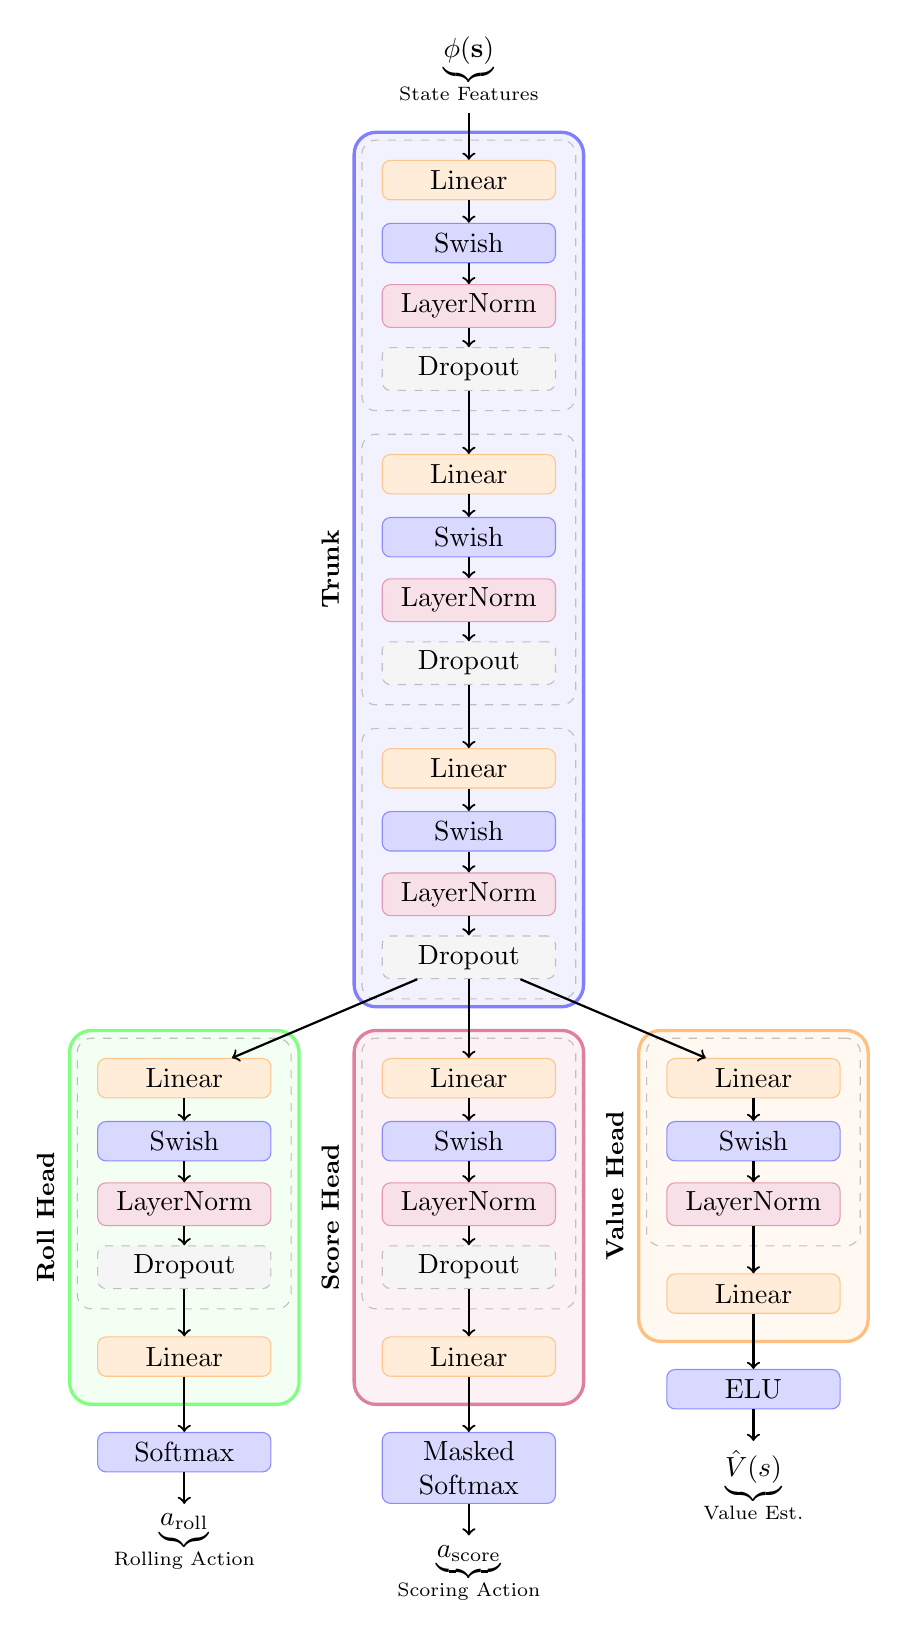
\begin{tikzpicture}[
        node distance=0.8cm,
        layer/.style={rectangle, draw, minimum width=2.2cm, minimum height=0.5cm, align=center, rounded corners=3pt},
        linear/.style={layer, fill=orange!15, draw=orange!45},
        norm/.style={layer, fill=purple!12, draw=purple!40},
        activation/.style={layer, fill=blue!15, draw=blue!45},
        dropout/.style={layer, fill=gray!8, draw=gray!50, dashed},
      ]

      % Input (outside the box)
      \node (input) {$\underbrace{\phi(\mathbf{s})}_{\text{State Features}}$};

      % ===== TRUNK BLOCK 1 =====
      \node[linear, below=0.6cm of input] (trunk1_linear) {Linear};
      \node[activation, below of=trunk1_linear] (trunk1_swish) {Swish};
      \node[norm, below of=trunk1_swish] (trunk1_ln) {LayerNorm};
      \node[dropout, below of=trunk1_ln] (trunk1_dropout) {Dropout};

      % ===== TRUNK BLOCK 2 =====
      \node[linear, below=0.8cm of trunk1_dropout] (trunk2_linear) {Linear};
      \node[activation, below of=trunk2_linear] (trunk2_swish) {Swish};
      \node[norm, below of=trunk2_swish] (trunk2_ln) {LayerNorm};
      \node[dropout, below of=trunk2_ln] (trunk2_dropout) {Dropout};

      % ===== TRUNK BLOCK 3 =====
      \node[linear, below=0.8cm of trunk2_dropout] (trunk3_linear) {Linear};
      \node[activation, below of=trunk3_linear] (trunk3_swish) {Swish};
      \node[norm, below of=trunk3_swish] (trunk3_ln) {LayerNorm};
      \node[dropout, below of=trunk3_ln] (trunk3_dropout) {Dropout};

      % ===== ROLL HEAD =====
      \node[linear, below left=1.0cm and 1.4cm of trunk3_dropout] (roll_linear) {Linear};
      \node[activation, below of=roll_linear] (roll_swish) {Swish};
      \node[norm, below of=roll_swish] (roll_ln) {LayerNorm};
      \node[dropout, below of=roll_ln] (roll_dropout) {Dropout};

      % ===== SCORE HEAD =====
      \node[linear, below=1.0cm of trunk3_dropout] (score_linear) {Linear};
      \node[activation, below of=score_linear] (score_swish) {Swish};
      \node[norm, below of=score_swish] (score_ln) {LayerNorm};
      \node[dropout, below of=score_ln] (score_dropout) {Dropout};

      % ===== VALUE HEAD =====
      \node[linear, below right=1.0cm and 1.4cm of trunk3_dropout] (value_linear) {Linear};
      \node[activation, below of=value_linear] (value_swish) {Swish};
      \node[norm, below of=value_swish] (value_ln) {LayerNorm};

      % ===== ROLL OUTPUT =====
      \node[linear, below=0.6cm of roll_dropout] (roll_out_linear) {Linear};
      \node[activation, below=0.7cm of roll_out_linear] (roll_out_softmax) {Softmax};
      \node[below=0.4cm of roll_out_softmax] (roll_out) {$\underbrace{a_{\mathrm{roll}}}_{\text{Rolling Action}}$};

      % ===== SCORE OUTPUT =====
      \node[linear, below=0.6cm of score_dropout] (score_out_linear) {Linear};
      \node[activation, below=0.7cm of score_out_linear] (score_out_softmax) {Masked\\Softmax};
      \node[below=0.4cm of score_out_softmax] (score_out) {$\underbrace{a_{\mathrm{score}}}_{\text{Scoring Action}}$};

      % ===== VALUE OUTPUT =====
      \node[linear, below=0.6cm of value_ln] (value_out_linear) {Linear};
      \node[activation, below=0.7cm of value_out_linear] (value_out_elu) {ELU};
      \node[below=0.4cm of value_out_elu] (value_out) {$\underbrace{\hat{V}(s)}_{\text{Value Est.}}$};

      % Surrounding boxes (drawn on background layer)
      \begin{scope}[on background layer]
        % Big trunk box (draw first, in background)
        \node[draw=blue!50, very thick, rectangle, rounded corners=8pt, fit={(trunk1_linear) (trunk1_swish) (trunk1_ln) (trunk1_dropout) (trunk2_linear) (trunk2_swish) (trunk2_ln) (trunk2_dropout) (trunk3_linear) (trunk3_swish) (trunk3_ln) (trunk3_dropout)}, inner sep=0.35cm, fill=blue!5] (trunk_box) {};

        % Roll head box (exclude output softmax)
        \node[draw=green!50, very thick, rectangle, rounded corners=8pt, fit={(roll_linear) (roll_swish) (roll_ln) (roll_dropout) (roll_out_linear)}, inner sep=0.35cm, fill=green!5] (roll_box) {};

        % Score head box (exclude output softmax)
        \node[draw=purple!50, very thick, rectangle, rounded corners=8pt, fit={(score_linear) (score_swish) (score_ln) (score_dropout) (score_out_linear)}, inner sep=0.35cm, fill=purple!5] (score_box) {};

        % Value head box (include output layers)
        \node[draw=orange!50, very thick, rectangle, rounded corners=8pt, fit={(value_linear) (value_swish) (value_ln) (value_out_linear)}, inner sep=0.35cm, fill=orange!5] (value_box) {};
      \end{scope}

      % Individual blocks with dashed grey outline (drawn on top)
      % Trunk Block 1
      \node[draw=gray!50, dashed, rectangle, rounded corners=5pt, fit={(trunk1_linear) (trunk1_swish) (trunk1_ln) (trunk1_dropout)}, inner sep=0.25cm, fill=none] {};

      % Trunk Block 2
      \node[draw=gray!50, dashed, rectangle, rounded corners=5pt, fit={(trunk2_linear) (trunk2_swish) (trunk2_ln) (trunk2_dropout)}, inner sep=0.25cm, fill=none] {};

      % Trunk Block 3
      \node[draw=gray!50, dashed, rectangle, rounded corners=5pt, fit={(trunk3_linear) (trunk3_swish) (trunk3_ln) (trunk3_dropout)}, inner sep=0.25cm, fill=none] {};

      % Roll Head inner block
      \node[draw=gray!50, dashed, rectangle, rounded corners=5pt, fit={(roll_linear) (roll_swish) (roll_ln) (roll_dropout)}, inner sep=0.25cm, fill=none] {};

      % Score Head inner block
      \node[draw=gray!50, dashed, rectangle, rounded corners=5pt, fit={(score_linear) (score_swish) (score_ln) (score_dropout)}, inner sep=0.25cm, fill=none] {};

      % Value Head inner block
      \node[draw=gray!50, dashed, rectangle, rounded corners=5pt, fit={(value_linear) (value_swish) (value_ln)}, inner sep=0.25cm, fill=none] {};

      % Labels for large boxes
      \node[left=0.05cm of trunk_box.west, rotate=90, anchor=south, font=\small\bfseries] {Trunk};
      \node[left=0.05cm of roll_box.west, rotate=90, anchor=south, font=\small\bfseries] {Roll Head};
      \node[left=0.05cm of score_box.west, rotate=90, anchor=south, font=\small\bfseries] {Score Head};
      \node[left=0.05cm of value_box.west, rotate=90, anchor=south, font=\small\bfseries] {Value Head};

      % Arrows - Trunk
      \draw[->, thick] (input) -- (trunk1_linear);
      \draw[->, thick] (trunk1_linear) -- (trunk1_swish);
      \draw[->, thick] (trunk1_swish) -- (trunk1_ln);
      \draw[->, thick] (trunk1_ln) -- (trunk1_dropout);
      \draw[->, thick] (trunk1_dropout) -- (trunk2_linear);
      \draw[->, thick] (trunk2_linear) -- (trunk2_swish);
      \draw[->, thick] (trunk2_swish) -- (trunk2_ln);
      \draw[->, thick] (trunk2_ln) -- (trunk2_dropout);
      \draw[->, thick] (trunk2_dropout) -- (trunk3_linear);
      \draw[->, thick] (trunk3_linear) -- (trunk3_swish);
      \draw[->, thick] (trunk3_swish) -- (trunk3_ln);
      \draw[->, thick] (trunk3_ln) -- (trunk3_dropout);

      % Arrows - Split to heads
      \draw[->, thick] (trunk3_dropout) -- (roll_linear);
      \draw[->, thick] (trunk3_dropout) -- (score_linear);
      \draw[->, thick] (trunk3_dropout) -- (value_linear);

      % Arrows - Roll head
      \draw[->, thick] (roll_linear) -- (roll_swish);
      \draw[->, thick] (roll_swish) -- (roll_ln);
      \draw[->, thick] (roll_ln) -- (roll_dropout);
      \draw[->, thick] (roll_dropout) -- (roll_out_linear);
      \draw[->, thick] (roll_out_linear) -- (roll_out_softmax);
      \draw[->, thick] (roll_out_softmax) -- (roll_out);

      % Arrows - Score head
      \draw[->, thick] (score_linear) -- (score_swish);
      \draw[->, thick] (score_swish) -- (score_ln);
      \draw[->, thick] (score_ln) -- (score_dropout);
      \draw[->, thick] (score_dropout) -- (score_out_linear);
      \draw[->, thick] (score_out_linear) -- (score_out_softmax);
      \draw[->, thick] (score_out_softmax) -- (score_out);

      % Arrows - Value head
      \draw[->, thick] (value_linear) -- (value_swish);
      \draw[->, thick] (value_swish) -- (value_ln);
      \draw[->, thick] (value_ln) -- (value_out_linear);
      \draw[->, thick] (value_out_linear) -- (value_out_elu);
      \draw[->, thick] (value_out_elu) -- (value_out);

    \end{tikzpicture}
  }
  \caption{Overall network architecture with shared trunk and three specialized heads}
  \label{fig:network-architecture}
\end{figure}

\subsubsection{Policy and Value Heads}
We utilize two distinct heads for the rolling and scoring actions, allowing the model to specialize in
each task \cite{tavakoli2018actionbranching, hausknecht2016parameterized}.
We also implement a value head. This outputs a scalar which is used as the baseline for REINFORCE and the value estimate for actor-critic methods.
Each of these networks has a fully connected hidden layer before the final output layer.

In the rolling action head, we use either 5 outputs with sigmoid activations for Bernoulli representation, or 32 outputs with softmax activations for the categorical representation.

In the scoring action head, we use 13 outputs with softmax activations for the categorical distribution over scoring categories.

For the value head, we use a single linear output, constrained with ELU activation to clamp negative value estimates \cite{clevert2016elu}, since negative rewards are not possible in \textit{Yahtzee}.

\subsubsection{Optimization \& Schedules}
We utilize the Adam optimizer \cite{kingma2014adam} with maximum learning rate $\alpha$, typically between $1\times 10^{-4}$ and $5\times 10^{-4}$.
To improve training stability, we utilize a warmup schedule over the first 5\% of training \cite{kalra-2024-warmup},
plateau for 70\% of training, and then linearly decay over the final 25\% of training steps to a minimum ratio $r_{\alpha}$ of the maximum \cite{defazio2023optimal, lyle2024normalization}.

\subsection{Entropy}
To encourage exploration, we also add an entropy bonus to the loss function  \cite{williams-peng-1991-function-optimization}. These are held
constant at the start of training then linearly decayed to a final value near the end of training. Different entropy bonuses were used for rolling and scoring actions,
as rolling actions had a tendency to collapse early in training.
Exploration is particularly important for Yahtzee, there are many stable suboptimal policies (e.g., exclusively going for the upper bonus, always going for Yahtzees, etc).
Once the model has figured out how to play the game, it quickly converges and won't explore other strategies as they often trade off short-term rewards for long-term gains.

We can define the entropy bonus as:
\begin{align}
  \mathcal{L}_{\mathrm{entropy}}(\theta)
  = &
  \underbrace{
    \overbrace{\beta_{\mathrm{roll}}}^{\text{weight}}
    \,
    \mathcal{H}\big[\pi_{\theta,\mathrm{roll}}(\cdot \mid s_t)\big]
  }_{\text{rolling action entropy}} \nonumber \\
    & +
  \underbrace{
    \overbrace{\beta_{\mathrm{score}}}^{\text{weight}}
    \,
    \mathcal{H}\big[\pi_{\theta,\mathrm{score}}(\cdot \mid s_t)\big]
  }_{\text{scoring action entropy}}
\end{align}

\subsubsection{Training Metrics}
To better understand training dynamics, we log several metrics during training.
To monitor the quality of the value network, we monitor explained variance \cite{schulman2016nutsbolts, schulman-2016-gae}.
To monitor for policy collapse, we track the policy entropy and KL divergence between policy updates \cite{schulman2016nutsbolts,schulman-2017-ppo},
mask diversity \cite{Hubara2021MaskDiversity},
and the top-k action frequency \cite{sun-etal-2025-curiosity}.
To monitor for learning stability, we track gradient norms and clip rate \cite{pascanu-2013-rnn-clipping, Engstrom2020ImplementationMatters}.
Gradient clipping is applied with threshold $\tau_{\mathrm{clip}}$ to prevent destabilizing updates.
To ensure advantages are well-conditioned, we track advantage mean and standard deviation \cite{Achiam2018SpinningUp}.
We also monitor standard training metrics such as average reward and loss values.

\subsection{Reinforcement Learning Algorithms}
\subsubsection{REINFORCE}
We first implement the REINFORCE algorithm \cite{williams-1992-reinforce} with baseline for single-turn optimization, then attempt to extend it to full-game optimization.
The baseline is the output of the value head, $V_{\phi}(\mathbf{s})$.
We collect trajectories in batches of $B$ games before computing gradient updates. Thus, the loss function is:

\begin{align}
  \mathcal{L}(\theta,\phi)
  = &
  \underbrace{
  \overbrace{- \log \big(\pi_\theta(a_t \mid s_t)\big)}^{\text{negative log likelihood}} \,
  \overbrace{\big(\hat{R}_t - V_\phi(s_t)\big)}^{\text{advantage }}
  }_{\text{policy loss}}                 \nonumber \\
    & +
  \underbrace{
  \overbrace{\lambda_V}^{\text{weight}}
  \|
  V_\phi(s_t) - \hat{R}_t\big
  \|_2
  }_{\text{value loss}}                  \nonumber \\
    & +
  \mathcal{L}_{\mathrm{entropy}(\theta)}
\end{align}

\subsubsection{Advantage Actor-Critic (A2C)}

Second, we utilize an episodic, one-step TD(0) Advantage Actor-Critic (A2C) method. Its loss is:

\begin{align}
  \delta_t
   & =
  \overbrace{r_t}^{\text{reward}}
  +
  \overbrace{\gamma V_\phi(s_{t+1})}^{\text{bootstrap}}
  -
  \overbrace{V_\phi(s_t)}^{\text{current estimate}}
\end{align}
\begin{align}
  \mathcal{L}_{\text{TD-AC}}(\theta,\phi)
  = &
  \underbrace{
  \overbrace{- \log \big(\pi_\theta(a_t \mid s_t)\big)}^{\text{negative log likelihood}}
  \,
  \overbrace{\delta_t}^{\text{TD-error}}
  }_{\text{policy loss}}                 \nonumber \\
    & +
  \underbrace{
  \overbrace{\lambda_V}^{\text{weight}}
  \,
  \big\|
  \delta_t
  \big\|_2^2
  }_{\text{value loss}}                  \nonumber \\
    & +
  \mathcal{L}_{\mathrm{entropy}(\theta)}
\end{align}

\subsubsection{PPO}
PPO improves on TD by utilizing a "surrogate" objective which clips large policy updates, improving training stability.
This allows for substantially larger batch sizes and learning rates \cite{schulman-2017-ppo}. The loss we use is:

\begin{align}
  r_t(\theta)
   & =
  \frac{
  \overbrace{\pi_\theta(a_t \mid s_t)}^{\text{current policy}}
  }{
  \underbrace{\pi_{\theta_{\text{old}}}(a_t \mid s_t)}_{\text{behavior policy}}
  }
\end{align}
\begin{align}
  \mathcal{L}(\theta,\phi)
  = &
  \underbrace{
    - \min \bigg\{
    \begin{aligned}
       & r_t(\theta)\,\hat{A}_t,                                                         \\
       & \operatorname{clip}\big(r_t(\theta), 1 - \epsilon, 1 + \epsilon\big)\,\hat{A}_t
    \end{aligned}
    \bigg\}
  }_{\text{policy loss}}                 \nonumber \\
    & +
  \underbrace{
  \overbrace{\lambda_V}^{\text{weight}}
  \big\|
  V_\phi(s_t) - \hat{R}_t
  \big\|_2^2
  }_{\text{value loss}}                  \nonumber \\
    & +
  \mathcal{L}_{\mathrm{entropy}(\theta)}
\end{align}

\subsubsection{Training Regimes}
We analyze several distinct training regimes for \textit{Yahtzee} agents:
\begin{enumerate*}[label=(\roman*)]
  \item REINFORCE directly on the single-turn optimization task and evaluating full-game performance
  \item REINFORCE, TD, and PPO directly on the full-game optimization task
        % \item transfer learning from single-turn to full-game optimization
        % \item behavioral cloning from an optimal DP agent
\end{enumerate*}.

\subsection{Evaluation Protocol}
During training, we run 1,000 game episodes every 5 epochs (1\% of training) to monitor progress.

For a model's final evaluation, we run 10,000 games, reporting the mean score and standard deviation.
For a typical variance $\sigma^2 \approx 50$, this generally gives us a standard error $\sigma / \sqrt{10000} = \pm 0.5$.
Likewise, we compute category statistics to analyze strategic preferences of different agents.

\section{Results}

\subsection{Single-Turn Results}
% <600-700 words>
\subsubsection{Baseline Single-Turn Performance}
For state representation, the baseline model utilizes:
$$\mathbf{x} = \phi(\mathbf{s}) = \big[\phi_{\mathrm{dice}}^{\mathrm{combined}}(\mathbf{d}), \phi_{\mathrm{cat}}(\mathbf{c}), \phi_{\mathrm{bonus}}(\mathbf{c}), \phi_{\mathrm{rolls}}(r)\big]$$
For outputs, it uses Bernoulli rolling actions and categorical scoring actions.
The single turn model has a short horizon (3 steps); REINFORCE was the natural choice here.
We trained on <X> single-turn episodes, using a batch size of <Y> episodes, for <Z> total gradient updates.

Although it does not nearly reach optimal performance, it performs surprisingly well over the full game; this is likely due to the high correlation between single-turn and full-game optimal actions.
However, we suspected target leakage (selecting parameters and architectures based on full-game performance) could also play a role and analyze the full-game vs. single-turn tradeoff in Section~\ref{sec:tradeoff-curve}.

\begin{figure}[H]
  \centering
  % Panel (a): Single-turn score
  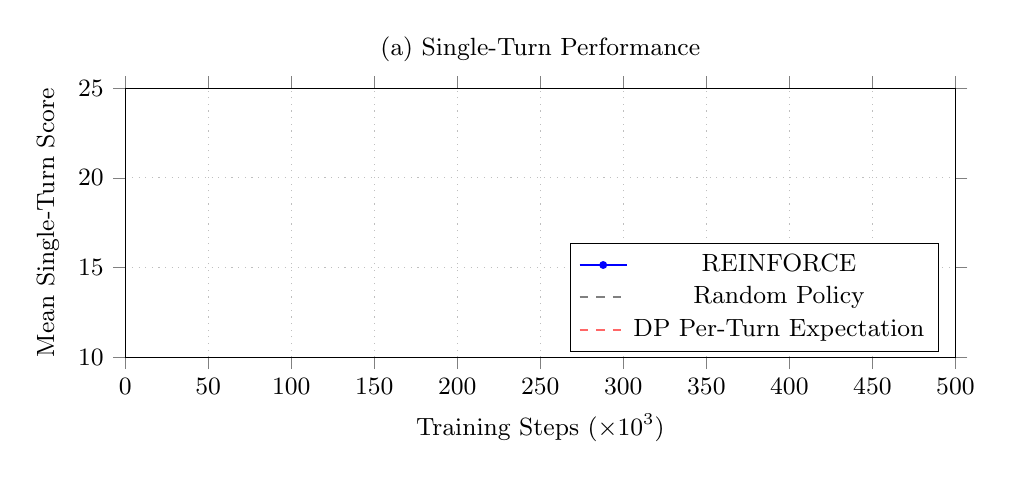
\begin{tikzpicture}
    \begin{axis}[
        width=\columnwidth,
        height=5cm,
        xlabel={Training Steps ($\times 10^3$)},
        ylabel={Mean Single-Turn Score},
        title={(a) Single-Turn Performance},
        xmin=0, xmax=500,
        ymin=10, ymax=25,
        grid=both,
        grid style={dotted},
        tick align=outside,
        tick label style={font=\small},
        label style={font=\small},
        title style={font=\small},
        legend style={at={(0.98,0.02)},anchor=south east,font=\small}
      ]

      % Main REINFORCE learning curve
      \addplot[
        thick,
        blue,
        mark=*,
        mark size=1pt,
        mark repeat=10
      ] coordinates {
          (0, 50)
          (50, 50)
          (100, 50)
          (150, 50)
          (200, 50)
          (250, 50)
          (300, 50)
          (350, 50)
          (400, 50)
          (450, 50)
          (500, 50)
        };
      \addlegendentry{REINFORCE}

      % Random policy baseline
      \addplot[
        dashed,
        gray,
        thick,
        domain=0:500
      ] {50};
      \addlegendentry{Random Policy}

      % DP per-turn expectation
      \addplot[
        dashed,
        red!60,
        thick,
        domain=0:500
      ] {50};
      \addlegendentry{DP Per-Turn Expectation}

    \end{axis}
  \end{tikzpicture}

  \vspace{0.5cm}

  % Panel (b): Full-game performance
  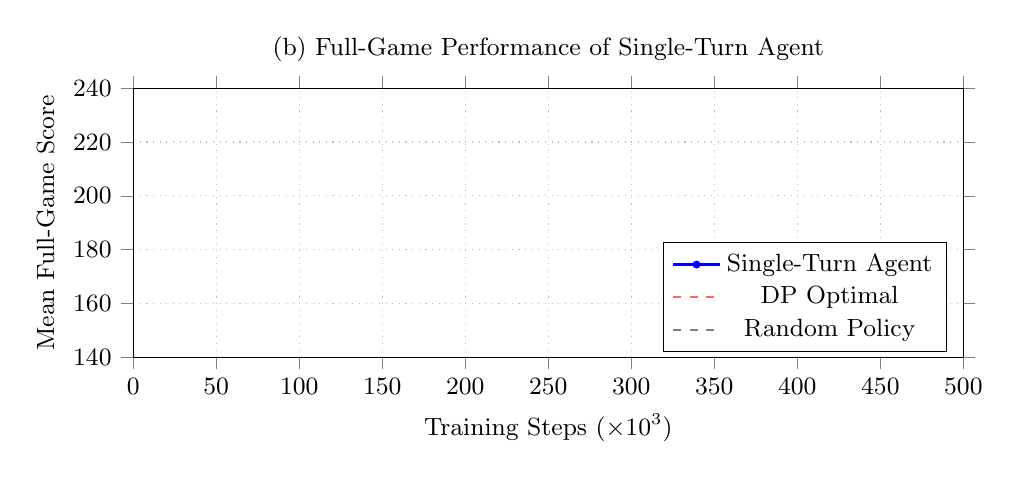
\begin{tikzpicture}
    \begin{axis}[
        width=\columnwidth,
        height=5cm,
        xlabel={Training Steps ($\times 10^3$)},
        ylabel={Mean Full-Game Score},
        title={(b) Full-Game Performance of Single-Turn Agent},
        xmin=0, xmax=500,
        ymin=140, ymax=240,
        grid=both,
        grid style={dotted},
        tick align=outside,
        tick label style={font=\small},
        label style={font=\small},
        title style={font=\small},
        legend style={at={(0.98,0.02)},anchor=south east,font=\small}
      ]

      % Full-game evaluation at checkpoints
      \addplot[
        thick,
        blue,
        mark=*,
        mark size=1pt,
        mark repeat=10
      ] coordinates {
          (0, 50)
          (50, 50)
          (100, 50)
          (150, 50)
          (200, 50)
          (250, 50)
          (300, 50)
          (350, 50)
          (400, 50)
          (450, 50)
          (500, 50)
        };
      \addlegendentry{Single-Turn Agent}

      % DP optimal baseline
      \addplot[
        dashed,
        red!60,
        thick,
        domain=0:500
      ] {50};
      \addlegendentry{DP Optimal}

      % Random policy baseline
      \addplot[
        dashed,
        gray,
        thick,
        domain=0:500
      ] {50};
      \addlegendentry{Random Policy}

    \end{axis}
  \end{tikzpicture}
  \caption{Single-turn agent training dynamics (placeholder data)}
  \label{fig:single-turn-learning-curve}
\end{figure}

\subsubsection{Single vs Full-game Tradeoff Curve}
\label{sec:tradeoff-curve}
To understand the tradeoff between single-turn and full-game performance, we ablated our model using small changes to various hyperparameters and captured
the resulting performance on both the primary single-turn score, as well as the auxiliary full-game score.
We expect that there is a Pareto frontier between these two objectives, and that some hyperparameter choices push performance towards one or the other.

\begin{figure}[H]
  \centering
  \begin{tikzpicture}
    \begin{axis}[
      width=\columnwidth,
      xlabel={$\bar{s}_{\text{single-turn}}$},
      ylabel={$\bar{s}_{\text{full-game}}$},
      title={Pareto Frontier of Single-Turn vs. Full-Game Performance},
      grid=both,
      grid style={dotted},
      tick align=outside,
      tick label style={font=\small},
      label style={font=\small},
      title style={font=\small},
      enlargelimits=0.05,
      legend style={at={(0.02,0.98)},anchor=north west,font=\small}
      ]

      % --- Scatter points: replace these with your data ---
      \addplot[
        only marks,
        mark=*,
        mark size=1.5pt
      ] coordinates {
          (50, 50)
          (50, 50)
          (50, 50)
          (50, 50)
          (50, 50)
        };
      \addlegendentry{RL configurations}

    \end{axis}
  \end{tikzpicture}
  \caption{Single-turn vs full-game performance (placeholder data)}
  \label{fig:pareto-frontier}
\end{figure}

\subsection{Full-Game Results}
% <600-700 words>
For the full-game model, we added several additional features to the state representation: $\phi_{\mathrm{progress}}(t)$ and $\phi_{\mathrm{potential}}(\mathbf{d}, \mathbf{c})$
while reusing the same underlying neural network architecture as the single-turn model. These additions were necessary to provide the model with sufficient context to make long-term strategic decisions.
While the $\phi_{\mathrm{progress}}(t)$ feature could be inferred from the scorecard, the model struggled to do so reliably.
We intentionally omitted the $\phi_{\mathrm{potential}}(\mathbf{d}, \mathbf{c})$ feature in single turn, as we wanted to ensure the model was capable of learning to reason about category potential on its own,
but found it to be necessary, especially with REINFORCE.

\subsubsection{Algorithm Comparison: REINFORCE, A2C, PPO}

REINFORCE proved challenging to optimize to high performance levels given our fixed training budget of 1 million full-game episodes (39 million steps).
It was highly sensitive to hyperparameters such as the critic coefficient, the entropy bonus, and batch size.
We also found that REINFORCE simply required more training data to converge at a reliable performance level across seeds; our implementation was trained on 1,000,000 games.
However, after optimization we were able to achieve reasonable performance, scoring a mean of <X> points on average over 10,000 full games.

<Talk about how A2C performs better than REINFORCE>

<Talk about how PPO surprisingly did not outperform A2C here, possible reasons why>

\begin{figure}[H]
  \centering
  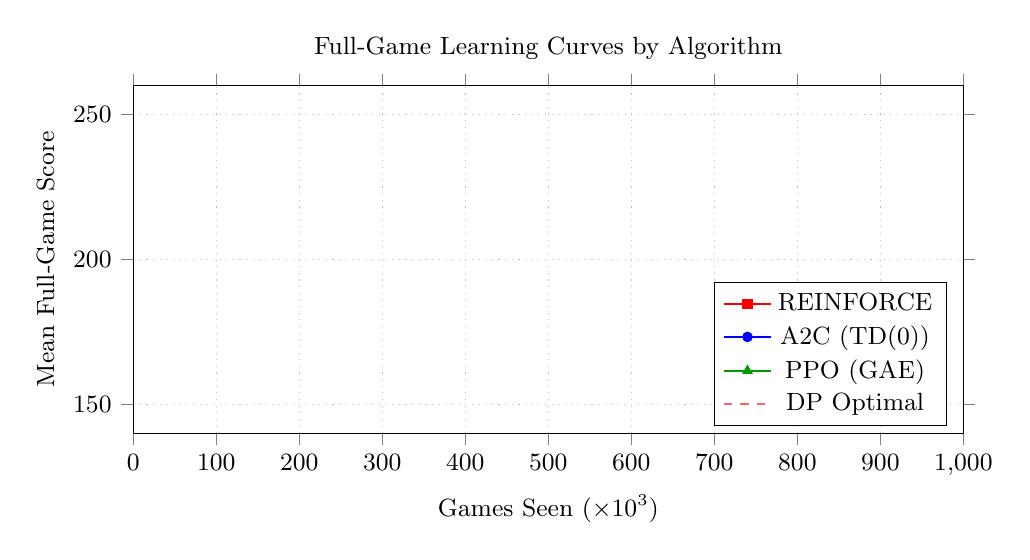
\begin{tikzpicture}
    \begin{axis}[
        width=\columnwidth,
        height=6cm,
        xlabel={Games Seen ($\times 10^3$)},
        ylabel={Mean Full-Game Score},
        title={Full-Game Learning Curves by Algorithm},
        xmin=0, xmax=1000,
        ymin=140, ymax=260,
        grid=both,
        grid style={dotted},
        tick align=outside,
        tick label style={font=\small},
        label style={font=\small},
        title style={font=\small},
        legend style={at={(0.98,0.02)},anchor=south east,font=\small}
      ]

      % REINFORCE learning curve
      \addplot[
        thick,
        red,
        mark=square*,
        mark size=1.5pt,
        mark repeat=20
      ] coordinates {
          (0, 50)
          (100, 50)
          (200, 50)
          (300, 50)
          (400, 50)
          (500, 50)
          (600, 50)
          (700, 50)
          (800, 50)
          (900, 50)
          (1000, 50)
        };
      \addlegendentry{REINFORCE}

      % A2C learning curve
      \addplot[
        thick,
        blue,
        mark=*,
        mark size=1.5pt,
        mark repeat=20
      ] coordinates {
          (0, 50)
          (100, 50)
          (200, 50)
          (300, 50)
          (400, 50)
          (500, 50)
          (600, 50)
          (700, 50)
          (800, 50)
          (900, 50)
          (1000, 50)
        };
      \addlegendentry{A2C (TD(0))}

      % PPO learning curve
      \addplot[
        thick,
        green!60!black,
        mark=triangle*,
        mark size=1.5pt,
        mark repeat=20
      ] coordinates {
          (0, 50)
          (100, 50)
          (200, 50)
          (300, 50)
          (400, 50)
          (500, 50)
          (600, 50)
          (700, 50)
          (800, 50)
          (900, 50)
          (1000, 50)
        };
      \addlegendentry{PPO (GAE)}

      % DP optimal baseline
      \addplot[
        dashed,
        red!60,
        thick,
        domain=0:1000
      ] {50};
      \addlegendentry{DP Optimal}

    \end{axis}
  \end{tikzpicture}
  \caption{Algorithm comparison learning curves (placeholder data)}
  \label{fig:full-game-learning-curves}
\end{figure}

\begin{figure}[H]
  \centering
  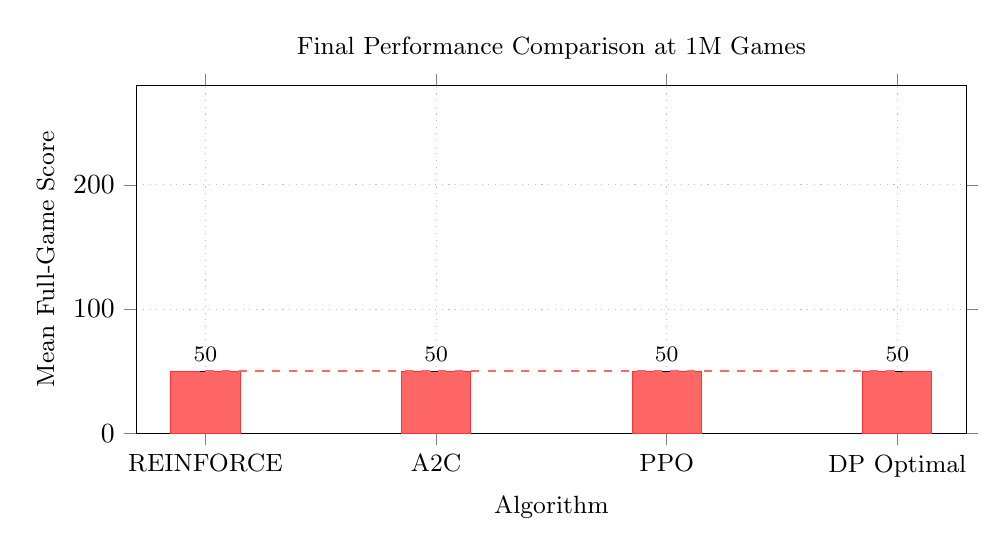
\begin{tikzpicture}
    \begin{axis}[
        ybar,
        width=\columnwidth,
        height=6cm,
        xlabel={Algorithm},
        ylabel={Mean Full-Game Score},
        title={Final Performance Comparison at 1M Games},
        symbolic x coords={REINFORCE, A2C, PPO, DP Optimal},
        xtick=data,
        xticklabel style={font=\small},
        ylabel style={font=\small},
        xlabel style={font=\small},
        title style={font=\small},
        bar width=25pt,
        ymin=0, ymax=280,
        grid=both,
        grid style={dotted},
        tick align=outside,
        nodes near coords,
        nodes near coords style={font=\footnotesize, anchor=south},
      ]

      \addplot[
        fill=red!60,
        draw=red!80,
        error bars/.cd,
        y dir=both,
        y explicit
      ] coordinates {
          (REINFORCE, 50) +- (0, 0)
          (A2C, 50) +- (0, 0)
          (PPO, 50) +- (0, 0)
          (DP Optimal, 50) +- (0, 0)
        };

      % Horizontal dashed line at DP optimal
      \draw[dashed, red!60, thick] (axis cs:REINFORCE,50) -- (axis cs:DP Optimal,50);

    \end{axis}
  \end{tikzpicture}
  \caption{Final performance, mean score (placeholder data)}
  \label{fig:final-performance-comparison}
\end{figure}

\begin{figure}[H]
  \centering
  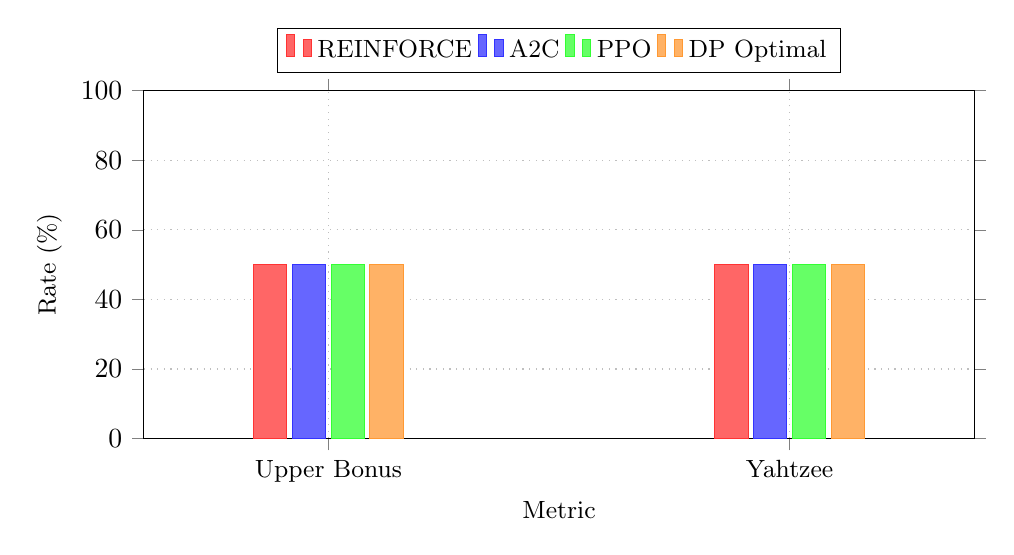
\begin{tikzpicture}
    \begin{axis}[
        ybar,
        width=\columnwidth,
        height=6cm,
        xlabel={Metric},
        ylabel={Rate (\%)},
        title={Bonus and Yahtzee Rates by Algorithm},
        symbolic x coords={Upper Bonus, Yahtzee},
        xtick=data,
        xticklabel style={font=\small},
        ylabel style={font=\small},
        xlabel style={font=\small},
        title style={font=\small},
        ymin=0, ymax=100,
        bar width=12pt,
        grid=both,
        grid style={dotted},
        tick align=outside,
        legend style={at={(0.5,1.05)},anchor=south,legend columns=4,font=\small},
        enlarge x limits=0.4,
      ]

      % REINFORCE
      \addplot[
        fill=red!60,
        draw=red!80
      ] coordinates {
          (Upper Bonus, 50)
          (Yahtzee, 50)
        };
      \addlegendentry{REINFORCE}

      % A2C
      \addplot[
        fill=blue!60,
        draw=blue!80
      ] coordinates {
          (Upper Bonus, 50)
          (Yahtzee, 50)
        };
      \addlegendentry{A2C}

      % PPO
      \addplot[
        fill=green!60,
        draw=green!80
      ] coordinates {
          (Upper Bonus, 50)
          (Yahtzee, 50)
        };
      \addlegendentry{PPO}

      % DP Optimal
      \addplot[
        fill=orange!60,
        draw=orange!80
      ] coordinates {
          (Upper Bonus, 50)
          (Yahtzee, 50)
        };
      \addlegendentry{DP Optimal}

    \end{axis}
  \end{tikzpicture}
  \caption{Bonus and Yahtzee achievement rates (placeholder data)}
  \label{fig:bonus-yahtzee-rates}
\end{figure}

\subsubsection{Representational Ablations}

<Discuss different state representations tested and their impact on performance>

\begin{figure}[H]
  \centering
  % Panel (a): Learning curves
  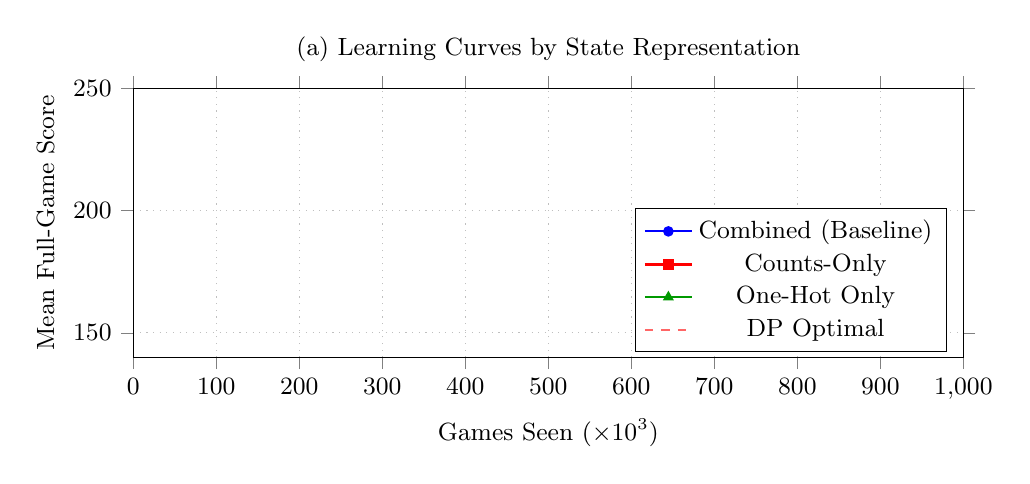
\begin{tikzpicture}
    \begin{axis}[
        width=\columnwidth,
        height=5cm,
        xlabel={Games Seen ($\times 10^3$)},
        ylabel={Mean Full-Game Score},
        title={(a) Learning Curves by State Representation},
        xmin=0, xmax=1000,
        ymin=140, ymax=250,
        grid=both,
        grid style={dotted},
        tick align=outside,
        tick label style={font=\small},
        label style={font=\small},
        title style={font=\small},
        legend style={at={(0.98,0.02)},anchor=south east,font=\small}
      ]

      % Combined (baseline)
      \addplot[
        thick,
        blue,
        mark=*,
        mark size=1.5pt,
        mark repeat=20
      ] coordinates {
          (0, 50)
          (100, 50)
          (200, 50)
          (300, 50)
          (400, 50)
          (500, 50)
          (600, 50)
          (700, 50)
          (800, 50)
          (900, 50)
          (1000, 50)
        };
      \addlegendentry{Combined (Baseline)}

      % Counts-only (simplest)
      \addplot[
        thick,
        red,
        mark=square*,
        mark size=1.5pt,
        mark repeat=20
      ] coordinates {
          (0, 50)
          (100, 50)
          (200, 50)
          (300, 50)
          (400, 50)
          (500, 50)
          (600, 50)
          (700, 50)
          (800, 50)
          (900, 50)
          (1000, 50)
        };
      \addlegendentry{Counts-Only}

      % One-hot only (potentially unstable or different)
      \addplot[
        thick,
        green!60!black,
        mark=triangle*,
        mark size=1.5pt,
        mark repeat=20
      ] coordinates {
          (0, 50)
          (100, 50)
          (200, 50)
          (300, 50)
          (400, 50)
          (500, 50)
          (600, 50)
          (700, 50)
          (800, 50)
          (900, 50)
          (1000, 50)
        };
      \addlegendentry{One-Hot Only}

      % DP optimal baseline
      \addplot[
        dashed,
        red!60,
        thick,
        domain=0:1000
      ] {50};
      \addlegendentry{DP Optimal}

    \end{axis}
  \end{tikzpicture}

  \vspace{0.5cm}

  % Panel (b): Bonus rate over training
  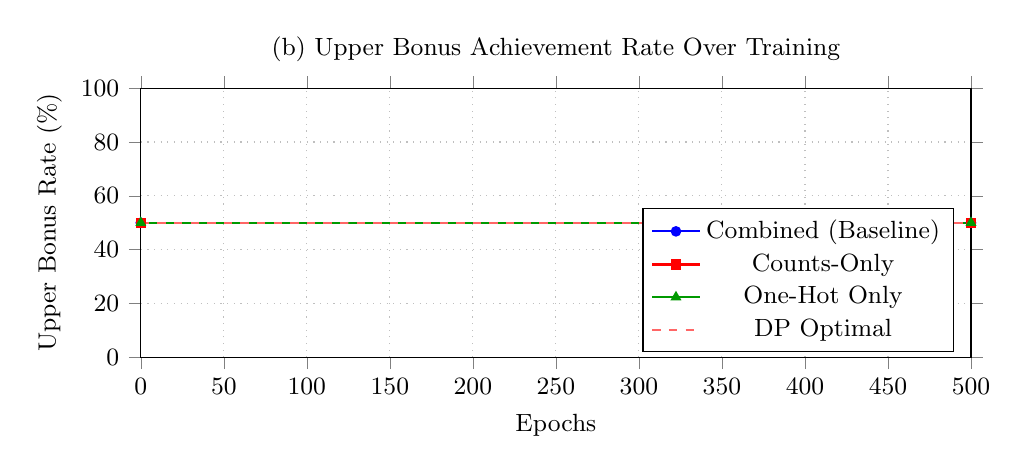
\begin{tikzpicture}
    \begin{axis}[
        width=\columnwidth,
        height=5cm,
        xlabel={Epochs},
        ylabel={Upper Bonus Rate (\%)},
        title={(b) Upper Bonus Achievement Rate Over Training},
        xmin=0, xmax=500,
        ymin=0, ymax=100,
        grid=both,
        grid style={dotted},
        tick align=outside,
        tick label style={font=\small},
        label style={font=\small},
        title style={font=\small},
        legend style={at={(0.98,0.02)},anchor=south east,font=\small}
      ]

      % Combined (baseline)
      \addplot[
        thick,
        blue,
        mark=*,
        mark size=1.5pt,
        mark repeat=10
      ] coordinates {
          (0, 50)
          (50, 50)
          (100, 50)
          (150, 50)
          (200, 50)
          (250, 50)
          (300, 50)
          (350, 50)
          (400, 50)
          (450, 50)
          (500, 50)
        };
      \addlegendentry{Combined (Baseline)}

      % Counts-only
      \addplot[
        thick,
        red,
        mark=square*,
        mark size=1.5pt,
        mark repeat=10
      ] coordinates {
          (0, 50)
          (50, 50)
          (100, 50)
          (150, 50)
          (200, 50)
          (250, 50)
          (300, 50)
          (350, 50)
          (400, 50)
          (450, 50)
          (500, 50)
        };
      \addlegendentry{Counts-Only}

      % One-hot only
      \addplot[
        thick,
        green!60!black,
        mark=triangle*,
        mark size=1.5pt,
        mark repeat=10
      ] coordinates {
          (0, 50)
          (50, 50)
          (100, 50)
          (150, 50)
          (200, 50)
          (250, 50)
          (300, 50)
          (350, 50)
          (400, 50)
          (450, 50)
          (500, 50)
        };
      \addlegendentry{One-Hot Only}

      % DP optimal baseline
      \addplot[
        dashed,
        red!60,
        thick,
        domain=0:500
      ] {50};
      \addlegendentry{DP Optimal}

    \end{axis}
  \end{tikzpicture}
  \caption{State representation ablation (placeholder data)}
  \label{fig:representation-ablation}
\end{figure}

\subsubsection{Architectural Ablations}

<Discuss network architecture choices and their impact>

\begin{figure}[H]
  \centering
  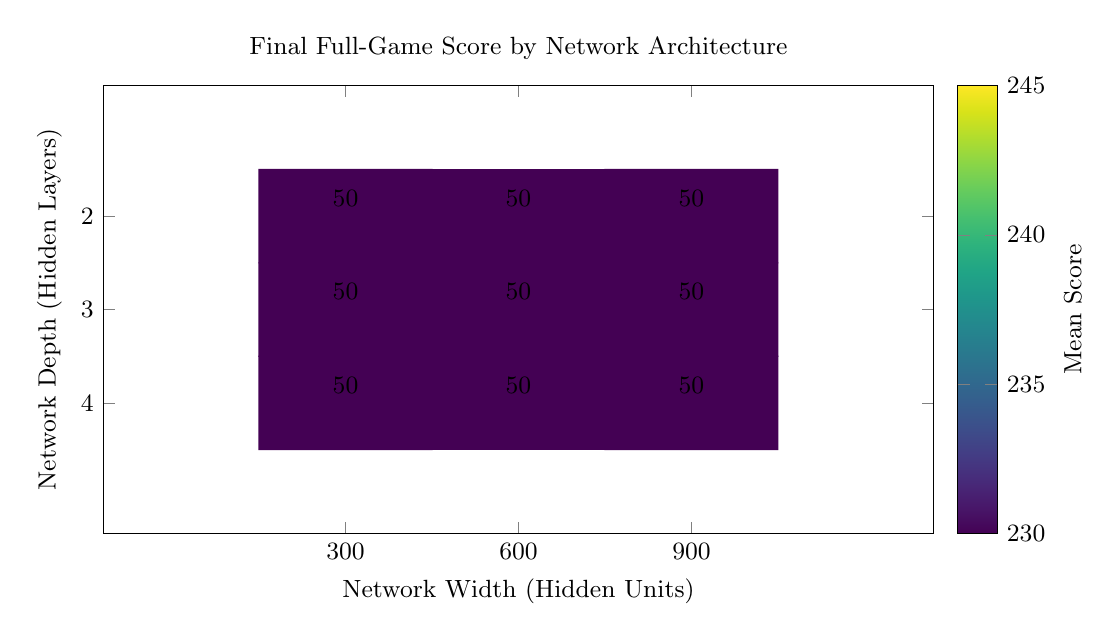
\begin{tikzpicture}
    \begin{axis}[
        width=\columnwidth,
        height=0.6\textwidth,
        xlabel={Network Width (Hidden Units)},
        ylabel={Network Depth (Hidden Layers)},
        title={Final Full-Game Score by Network Architecture},
        colormap/viridis,
        colorbar,
        colorbar style={
            ylabel={Mean Score},
            ylabel style={font=\small},
            ticklabel style={font=\small}
          },
        xlabel style={font=\small},
        ylabel style={font=\small},
        title style={font=\small},
        xtick={1,2,3},
        xticklabels={300, 600, 900},
        ytick={1,2,3},
        yticklabels={2, 3, 4},
        xticklabel style={font=\small},
        yticklabel style={font=\small},
        enlargelimits=0.3,
        point meta min=230,
        point meta max=245,
        nodes near coords,
        nodes near coords style={font=\small, color=black},
        every node near coord/.append style={xshift=0pt, yshift=0pt},
      ]

      \addplot[
        matrix plot,
        mesh/cols=3,
        point meta=explicit
      ] table[meta=score] {
          x y score
          1 1 50
          2 1 50
          3 1 50
          1 2 50
          2 2 50
          3 2 50
          1 3 50
          2 3 50
          3 3 50
        };

    \end{axis}
  \end{tikzpicture}
  \caption{Network architecture ablation (placeholder data)}
  \label{fig:architecture-heatmap}
\end{figure}

<Discuss LayerNorm's impact on training stability and performance>

\begin{figure}[H]
  \centering
  % Panel (a): Learning curves
  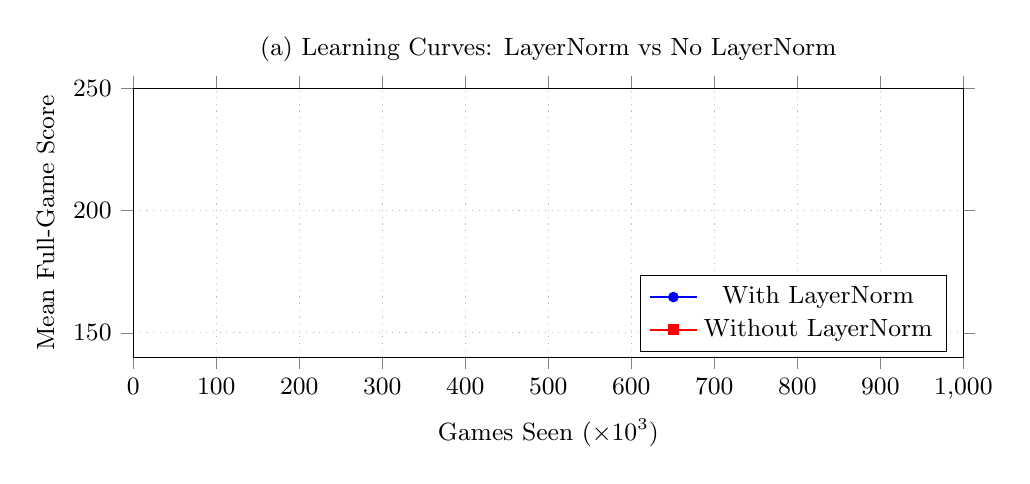
\begin{tikzpicture}
    \begin{axis}[
        width=\columnwidth,
        height=5cm,
        xlabel={Games Seen ($\times 10^3$)},
        ylabel={Mean Full-Game Score},
        title={(a) Learning Curves: LayerNorm vs No LayerNorm},
        xmin=0, xmax=1000,
        ymin=140, ymax=250,
        grid=both,
        grid style={dotted},
        tick align=outside,
        tick label style={font=\small},
        label style={font=\small},
        title style={font=\small},
        legend style={at={(0.98,0.02)},anchor=south east,font=\small}
      ]

      % With LayerNorm
      \addplot[
        thick,
        blue,
        mark=*,
        mark size=1.5pt,
        mark repeat=20
      ] coordinates {
          (0, 50)
          (100, 50)
          (200, 50)
          (300, 50)
          (400, 50)
          (500, 50)
          (600, 50)
          (700, 50)
          (800, 50)
          (900, 50)
          (1000, 50)
        };
      \addlegendentry{With LayerNorm}

      % Without LayerNorm
      \addplot[
        thick,
        red,
        mark=square*,
        mark size=1.5pt,
        mark repeat=20
      ] coordinates {
          (0, 50)
          (100, 50)
          (200, 50)
          (300, 50)
          (400, 50)
          (500, 50)
          (600, 50)
          (700, 50)
          (800, 50)
          (900, 50)
          (1000, 50)
        };
      \addlegendentry{Without LayerNorm}

    \end{axis}
  \end{tikzpicture}

  \vspace{0.5cm}

  % Panel (b): Explained variance
  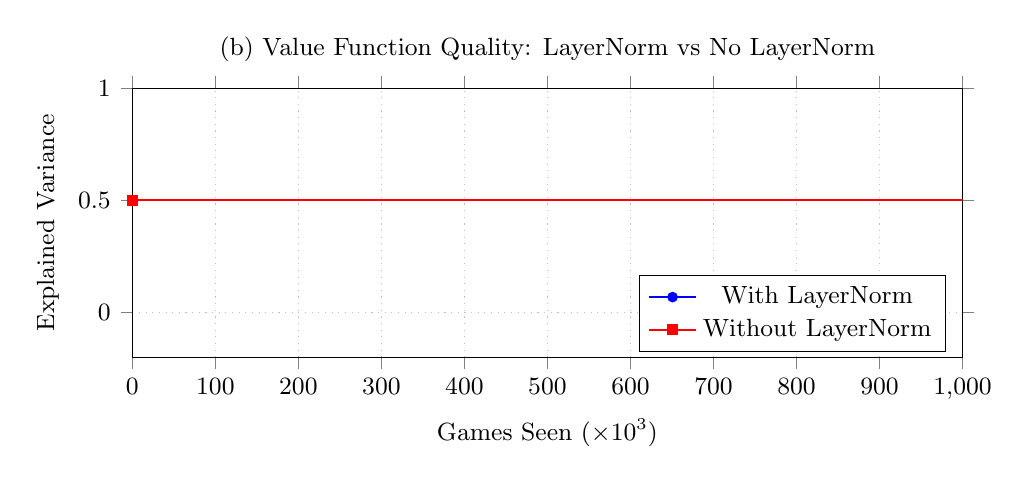
\begin{tikzpicture}
    \begin{axis}[
        width=\columnwidth,
        height=5cm,
        xlabel={Games Seen ($\times 10^3$)},
        ylabel={Explained Variance},
        title={(b) Value Function Quality: LayerNorm vs No LayerNorm},
        xmin=0, xmax=1000,
        ymin=-0.2, ymax=1.0,
        grid=both,
        grid style={dotted},
        tick align=outside,
        tick label style={font=\small},
        label style={font=\small},
        title style={font=\small},
        legend style={at={(0.98,0.02)},anchor=south east,font=\small}
      ]

      % With LayerNorm
      \addplot[
        thick,
        blue,
        mark=*,
        mark size=1.5pt,
        mark repeat=20
      ] coordinates {
          (0, 0.5)
          (100, 0.5)
          (200, 0.5)
          (300, 0.5)
          (400, 0.5)
          (500, 0.5)
          (600, 0.5)
          (700, 0.5)
          (800, 0.5)
          (900, 0.5)
          (1000, 0.5)
        };
      \addlegendentry{With LayerNorm}

      % Without LayerNorm
      \addplot[
        thick,
        red,
        mark=square*,
        mark size=1.5pt,
        mark repeat=20
      ] coordinates {
          (0, 0.5)
          (100, 0.5)
          (200, 0.5)
          (300, 0.5)
          (400, 0.5)
          (500, 0.5)
          (600, 0.5)
          (700, 0.5)
          (800, 0.5)
          (900, 0.5)
          (1000, 0.5)
        };
      \addlegendentry{Without LayerNorm}

    \end{axis}
  \end{tikzpicture}
  \caption{LayerNorm ablation (placeholder data)}
  \label{fig:layernorm-ablation}
\end{figure}

\subsubsection{Credit Assignment: TD(0) vs GAE}

<Discuss the effect of GAE lambda on performance and training dynamics>

\begin{figure}[H]
  \centering
  % Panel (a): Mean score vs lambda
  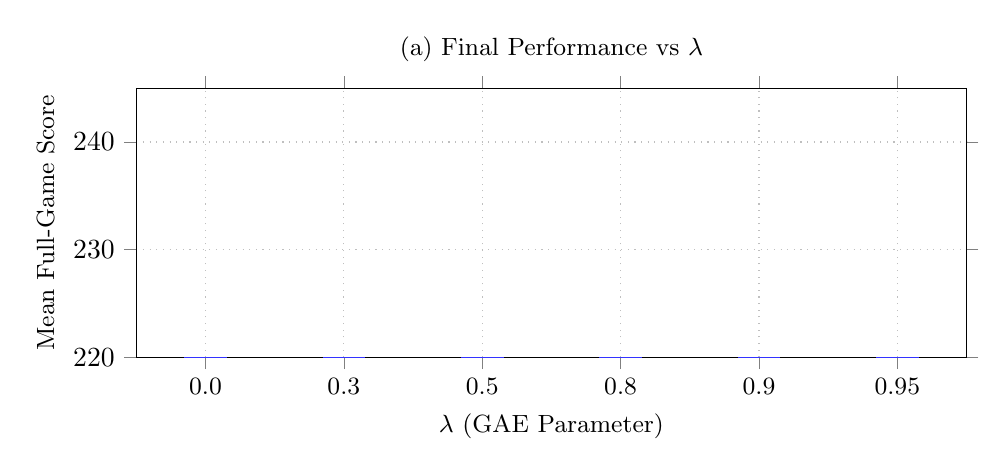
\begin{tikzpicture}
    \begin{axis}[
        ybar,
        width=\columnwidth,
        height=5cm,
        xlabel={$\lambda$ (GAE Parameter)},
        ylabel={Mean Full-Game Score},
        title={(a) Final Performance vs $\lambda$},
        symbolic x coords={0.0, 0.3, 0.5, 0.8, 0.9, 0.95},
        xtick=data,
        xticklabel style={font=\small},
        ylabel style={font=\small},
        xlabel style={font=\small},
        title style={font=\small},
        bar width=15pt,
        ymin=220, ymax=245,
        grid=both,
        grid style={dotted},
        tick align=outside,
        nodes near coords,
        nodes near coords style={font=\footnotesize, anchor=south},
      ]

      \addplot[
        fill=blue!60,
        draw=blue!80,
        error bars/.cd,
        y dir=both,
        y explicit
      ] coordinates {
          (0.0, 50) +- (0, 0)
          (0.3, 50) +- (0, 0)
          (0.5, 50) +- (0, 0)
          (0.8, 50) +- (0, 0)
          (0.9, 50) +- (0, 0)
          (0.95, 50) +- (0, 0)
        };

    \end{axis}
  \end{tikzpicture}

  \vspace{0.5cm}

  % Panel (b): Bonus rate vs lambda
  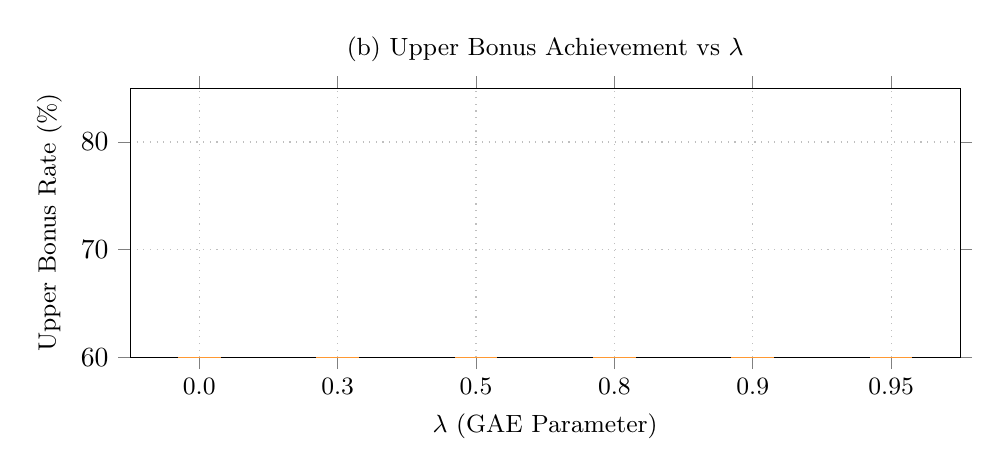
\begin{tikzpicture}
    \begin{axis}[
        ybar,
        width=\columnwidth,
        height=5cm,
        xlabel={$\lambda$ (GAE Parameter)},
        ylabel={Upper Bonus Rate (\%)},
        title={(b) Upper Bonus Achievement vs $\lambda$},
        symbolic x coords={0.0, 0.3, 0.5, 0.8, 0.9, 0.95},
        xtick=data,
        xticklabel style={font=\small},
        ylabel style={font=\small},
        xlabel style={font=\small},
        title style={font=\small},
        bar width=15pt,
        ymin=60, ymax=85,
        grid=both,
        grid style={dotted},
        tick align=outside,
        nodes near coords,
        nodes near coords style={font=\footnotesize, anchor=south},
      ]

      \addplot[
        fill=orange!60,
        draw=orange!80,
        error bars/.cd,
        y dir=both,
        y explicit
      ] coordinates {
          (0.0, 50) +- (0, 0)
          (0.3, 50) +- (0, 0)
          (0.5, 50) +- (0, 0)
          (0.8, 50) +- (0, 0)
          (0.9, 50) +- (0, 0)
          (0.95, 50) +- (0, 0)
        };

    \end{axis}
  \end{tikzpicture}
  \caption{GAE lambda ablation (placeholder data)}
  \label{fig:gae-lambda-ablation}
\end{figure}

\subsubsection{Entropy Sensitivity}

<Discuss the importance of entropy scheduling for exploration and policy collapse prevention>

\begin{table}[H]
  \centering
  \small
  \caption{Entropy regime definitions}
  \label{tab:entropy-regime-definitions}
  \begin{tabular}{lcc}
    \hline
    \textbf{Regime} & $\beta_{\mathrm{roll}}$   & $\beta_{\mathrm{score}}$ \\
    \hline
    Low Entropy     & 0.005 $\rightarrow$ 0.001 & 0.01 $\rightarrow$ 0.002 \\
    Baseline        & 0.01 $\rightarrow$ 0.002  & 0.02 $\rightarrow$ 0.005 \\
    High Entropy    & 0.02 $\rightarrow$ 0.005  & 0.04 $\rightarrow$ 0.01  \\
    \hline
  \end{tabular}
\end{table}

\begin{figure}[H]
  \centering
  % Panel (a): Rolling-head entropy
  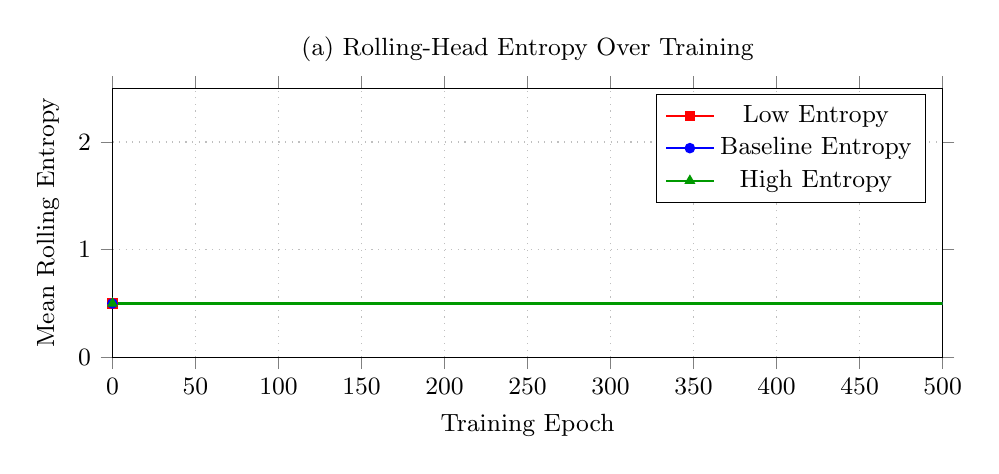
\begin{tikzpicture}
    \begin{axis}[
        width=\columnwidth,
        height=5cm,
        xlabel={Training Epoch},
        ylabel={Mean Rolling Entropy},
        title={(a) Rolling-Head Entropy Over Training},
        xmin=0, xmax=500,
        ymin=0, ymax=2.5,
        grid=both,
        grid style={dotted},
        tick align=outside,
        tick label style={font=\small},
        label style={font=\small},
        title style={font=\small},
        legend style={at={(0.98,0.98)},anchor=north east,font=\small}
      ]

      % Low entropy
      \addplot[
        thick,
        red,
        mark=square*,
        mark size=1.5pt,
        mark repeat=20
      ] coordinates {
          (0, 0.5)
          (50, 0.5)
          (100, 0.5)
          (150, 0.5)
          (200, 0.5)
          (250, 0.5)
          (300, 0.5)
          (350, 0.5)
          (400, 0.5)
          (450, 0.5)
          (500, 0.5)
        };
      \addlegendentry{Low Entropy}

      % Baseline entropy
      \addplot[
        thick,
        blue,
        mark=*,
        mark size=1.5pt,
        mark repeat=20
      ] coordinates {
          (0, 0.5)
          (50, 0.5)
          (100, 0.5)
          (150, 0.5)
          (200, 0.5)
          (250, 0.5)
          (300, 0.5)
          (350, 0.5)
          (400, 0.5)
          (450, 0.5)
          (500, 0.5)
        };
      \addlegendentry{Baseline Entropy}

      % High entropy
      \addplot[
        thick,
        green!60!black,
        mark=triangle*,
        mark size=1.5pt,
        mark repeat=20
      ] coordinates {
          (0, 0.5)
          (50, 0.5)
          (100, 0.5)
          (150, 0.5)
          (200, 0.5)
          (250, 0.5)
          (300, 0.5)
          (350, 0.5)
          (400, 0.5)
          (450, 0.5)
          (500, 0.5)
        };
      \addlegendentry{High Entropy}

    \end{axis}
  \end{tikzpicture}

  \vspace{0.5cm}

  % Panel (b): Scoring-head entropy
  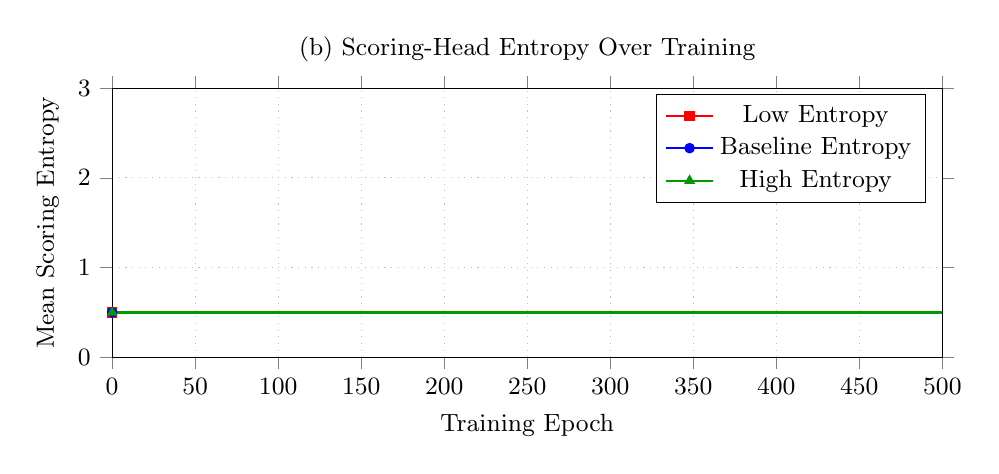
\begin{tikzpicture}
    \begin{axis}[
        width=\columnwidth,
        height=5cm,
        xlabel={Training Epoch},
        ylabel={Mean Scoring Entropy},
        title={(b) Scoring-Head Entropy Over Training},
        xmin=0, xmax=500,
        ymin=0, ymax=3.0,
        grid=both,
        grid style={dotted},
        tick align=outside,
        tick label style={font=\small},
        label style={font=\small},
        title style={font=\small},
        legend style={at={(0.98,0.98)},anchor=north east,font=\small}
      ]

      % Low entropy
      \addplot[
        thick,
        red,
        mark=square*,
        mark size=1.5pt,
        mark repeat=20
      ] coordinates {
          (0, 0.5)
          (50, 0.5)
          (100, 0.5)
          (150, 0.5)
          (200, 0.5)
          (250, 0.5)
          (300, 0.5)
          (350, 0.5)
          (400, 0.5)
          (450, 0.5)
          (500, 0.5)
        };
      \addlegendentry{Low Entropy}

      % Baseline entropy
      \addplot[
        thick,
        blue,
        mark=*,
        mark size=1.5pt,
        mark repeat=20
      ] coordinates {
          (0, 0.5)
          (50, 0.5)
          (100, 0.5)
          (150, 0.5)
          (200, 0.5)
          (250, 0.5)
          (300, 0.5)
          (350, 0.5)
          (400, 0.5)
          (450, 0.5)
          (500, 0.5)
        };
      \addlegendentry{Baseline Entropy}

      % High entropy
      \addplot[
        thick,
        green!60!black,
        mark=triangle*,
        mark size=1.5pt,
        mark repeat=20
      ] coordinates {
          (0, 0.5)
          (50, 0.5)
          (100, 0.5)
          (150, 0.5)
          (200, 0.5)
          (250, 0.5)
          (300, 0.5)
          (350, 0.5)
          (400, 0.5)
          (450, 0.5)
          (500, 0.5)
        };
      \addlegendentry{High Entropy}

    \end{axis}
  \end{tikzpicture}
  \caption{Entropy schedules (placeholder data)}
  \label{fig:entropy-schedules}
\end{figure}

\begin{table}[H]
  \centering
  \small
  \caption{Entropy regime performance (placeholder data)}
  \label{tab:entropy-regimes}
  \begin{tabular}{lccc}
    \hline
    \textbf{Regime} & \textbf{Mean Score} & \textbf{Bonus \%} & \textbf{Yahtzee \%} \\
    \hline
    Low Entropy     & $<X> \pm <Y>$       & <X>               & <Y>                 \\
    Baseline        & $<X> \pm <Y>$       & <X>               & <Y>                 \\
    High Entropy    & $<X> \pm <Y>$       & <X>               & <Y>                 \\
    \hline
  \end{tabular}
\end{table}

<Discuss how low entropy causes early policy collapse (lower scores and bonus rates), baseline achieves best performance, and high entropy maintains exploration but slows learning>

\subsubsection{Summary}

\begin{table*}[t]
  \centering
  \small
  \caption{Full-game performance summary (placeholder data)}
  \label{tab:full-game-summary}
  \begin{tabular}{lcccccc}
    \hline
    \textbf{Algorithm}               & \textbf{Training Budget} & \textbf{Mean Score} & \textbf{Std Dev} & \textbf{Bonus Rate (\%)} & \textbf{Yahtzee Rate (\%)} & \textbf{$\geq$250 (\%)} \\
    \hline
    DP Optimal                       & --                       & $<X>$               & --               & $<X>$                    & $<Y>$                      & $<Z>$                   \\
    A2C (TD(0), best config)         & 1M games                 & $<X>$               & $<Y>$            & $<X>$                    & $<Y>$                      & $<Z>$                   \\
    PPO ($\lambda=0.5$, best config) & 1M games                 & $<X>$               & $<Y>$            & $<X>$                    & $<Y>$                      & $<Z>$                   \\
    REINFORCE (full-game)            & 1M games                 & $<X>$               & $<Y>$            & $<X>$                    & $<Y>$                      & $<Z>$                   \\
    Single-Turn REINFORCE (rollout)  & 500K games               & $<X>$               & $<Y>$            & $<X>$                    & $<Y>$                      & $<Z>$                   \\
    \hline
  \end{tabular}
\end{table*}

\begin{table}[H]
  \centering
  \small
  \caption{Score distribution (placeholder data)}
  \label{tab:dp-score-distribution}
  \begin{tabular}{cc}
    \hline
    \textbf{$n$} & \textbf{$P(\text{score} \geq n)$} \\
    \hline
    50           & $<X>$                             \\
    100          & $<X>$                             \\
    150          & $<X>$                             \\
    200          & $<X>$                             \\
    250          & $<X>$                             \\
    300          & $<X>$                             \\
    400          & $<X>$                             \\
    500          & $<X>$                             \\
    750          & $<X>$                             \\
    1000         & $<X>$                             \\
    1250         & $<X>$                             \\
    1500         & $<X>$                             \\
    \hline
  \end{tabular}
\end{table}

<Summarize full-game results and key findings>

\subsection{Policy Analysis}
% <300-500 words>
\subsubsection{Category Usage}
<Bar chart showing average score per category for different agents>

<Summarize full-game results and key findings>
\begin{figure}[H]
  \centering
  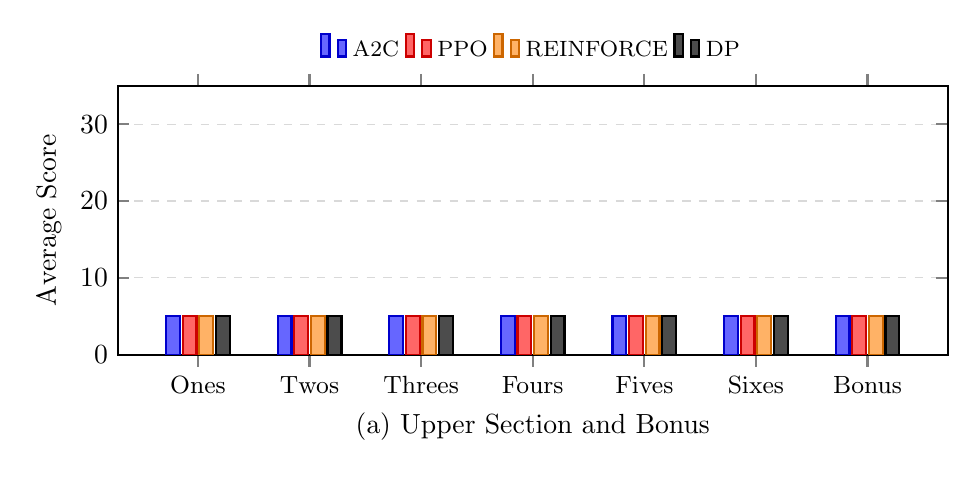
\begin{tikzpicture}
    % Panel (a): Upper Section + Bonus
    \begin{axis}[
        ybar=1pt,
        width=\columnwidth,
        height=5cm,
        bar width=5pt,
        symbolic x coords={Ones,Twos,Threes,Fours,Fives,Sixes,Bonus},
        xtick=data,
        xticklabel style={font=\small},
        ylabel={Average Score},
        xlabel={(a) Upper Section and Bonus},
        ymin=0,
        ymax=35,
        ymajorgrids=true,
        grid style={dashed,gray!30},
        legend style={
            at={(0.5,1.05)},
            anchor=south,
            legend columns=4,
            font=\footnotesize,
            draw=none,
            fill=none
          },
        enlarge x limits=0.12,
        axis line style={thick},
        tick style={thick},
      ]

      % A2C
      \addplot[fill=blue!60, draw=blue!80!black, thick] coordinates {
          (Ones,   5) (Twos,   5) (Threes, 5) (Fours,  5)
          (Fives,  5) (Sixes,  5) (Bonus,  5)
        };

      % PPO
      \addplot[fill=red!60, draw=red!80!black, thick] coordinates {
          (Ones,   5) (Twos,   5) (Threes, 5) (Fours,  5)
          (Fives,  5) (Sixes,  5) (Bonus,  5)
        };

      % REINFORCE
      \addplot[fill=orange!60, draw=orange!80!black, thick] coordinates {
          (Ones,   5) (Twos,   5) (Threes, 5) (Fours,  5)
          (Fives,  5) (Sixes,  5) (Bonus,  5)
        };

      % DP
      \addplot[fill=black!70, draw=black, thick] coordinates {
          (Ones,   5) (Twos,   5) (Threes, 5) (Fours,  5)
          (Fives,  5) (Sixes,  5) (Bonus,  5)
        };

      \legend{A2C,PPO,REINFORCE,DP}

    \end{axis}
  \end{tikzpicture}

  \vspace{0.4cm}

  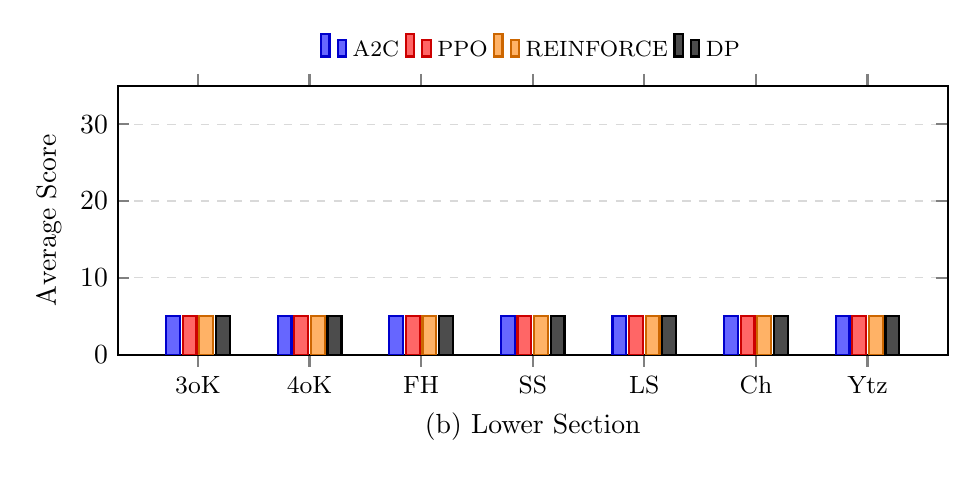
\begin{tikzpicture}
    % Panel (b): Lower Section
    \begin{axis}[
        ybar=1pt,
        width=\columnwidth,
        height=5cm,
        bar width=5pt,
        symbolic x coords={3oK,4oK,FH,SS,LS,Ch,Ytz},
        xtick=data,
        xticklabel style={font=\small},
        ylabel={Average Score},
        xlabel={(b) Lower Section},
        ymin=0,
        ymax=35,
        ymajorgrids=true,
        grid style={dashed,gray!30},
        legend style={
            at={(0.5,1.05)},
            anchor=south,
            legend columns=4,
            font=\footnotesize,
            draw=none,
            fill=none
          },
        enlarge x limits=0.12,
        axis line style={thick},
        tick style={thick},
      ]

      % A2C
      \addplot[fill=blue!60, draw=blue!80!black, thick] coordinates {
          (3oK,  5) (4oK,  5) (FH,   5) (SS,   5)
          (LS,   5) (Ch,   5) (Ytz,  5)
        };

      % PPO
      \addplot[fill=red!60, draw=red!80!black, thick] coordinates {
          (3oK,  5) (4oK,  5) (FH,   5) (SS,   5)
          (LS,   5) (Ch,   5) (Ytz,  5)
        };

      % REINFORCE
      \addplot[fill=orange!60, draw=orange!80!black, thick] coordinates {
          (3oK,  5) (4oK,  5) (FH,   5) (SS,   5)
          (LS,   5) (Ch,   5) (Ytz,  5)
        };

      % DP
      \addplot[fill=black!70, draw=black, thick] coordinates {
          (3oK,  5) (4oK,  5) (FH,   5) (SS,   5)
          (LS,   5) (Ch,   5) (Ytz,  5)
        };

      \legend{A2C,PPO,REINFORCE,DP}

    \end{axis}
  \end{tikzpicture}
  \caption{Average score per category (placeholder data)}
  \label{fig:category-scores}
\end{figure}

<table comparison against DP optimal solutions>

\subsubsection{Strategy Comparison Across Agents}

\begin{figure}[H]
  \centering
  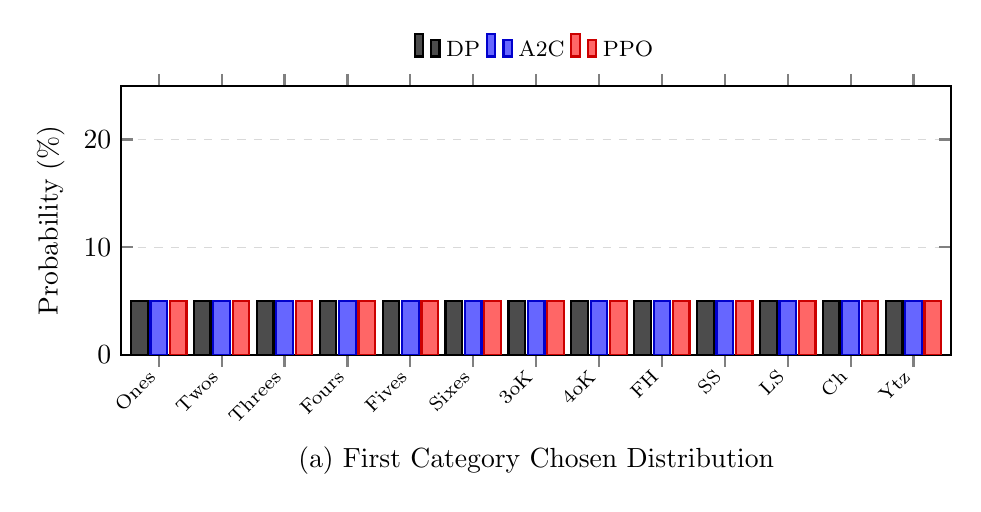
\begin{tikzpicture}
    % Panel (a): First Category Chosen Distribution
    \begin{axis}[
        ybar=1pt,
        width=\columnwidth,
        height=5cm,
        bar width=6pt,
        symbolic x coords={Ones,Twos,Threes,Fours,Fives,Sixes,3oK,4oK,FH,SS,LS,Ch,Ytz},
        xtick=data,
        xticklabel style={font=\scriptsize, rotate=45, anchor=east},
        ylabel={Probability (\%)},
        xlabel={(a) First Category Chosen Distribution},
        ymin=0,
        ymax=25,
        ymajorgrids=true,
        grid style={dashed,gray!30},
        legend style={
            at={(0.5,1.05)},
            anchor=south,
            legend columns=3,
            font=\footnotesize,
            draw=none,
            fill=none
          },
        enlarge x limits=0.05,
        axis line style={thick},
        tick style={thick},
      ]

      % DP
      \addplot[fill=black!70, draw=black, thick] coordinates {
          (Ones,5) (Twos,5) (Threes,5) (Fours,5) (Fives,5) (Sixes,5)
          (3oK,5) (4oK,5) (FH,5) (SS,5) (LS,5) (Ch,5) (Ytz,5)
        };

      % A2C
      \addplot[fill=blue!60, draw=blue!80!black, thick] coordinates {
          (Ones,5) (Twos,5) (Threes,5) (Fours,5) (Fives,5) (Sixes,5)
          (3oK,5) (4oK,5) (FH,5) (SS,5) (LS,5) (Ch,5) (Ytz,5)
        };

      % PPO
      \addplot[fill=red!60, draw=red!80!black, thick] coordinates {
          (Ones,5) (Twos,5) (Threes,5) (Fours,5) (Fives,5) (Sixes,5)
          (3oK,5) (4oK,5) (FH,5) (SS,5) (LS,5) (Ch,5) (Ytz,5)
        };

      \legend{DP,A2C,PPO}

    \end{axis}
  \end{tikzpicture}

  \vspace{0.4cm}

  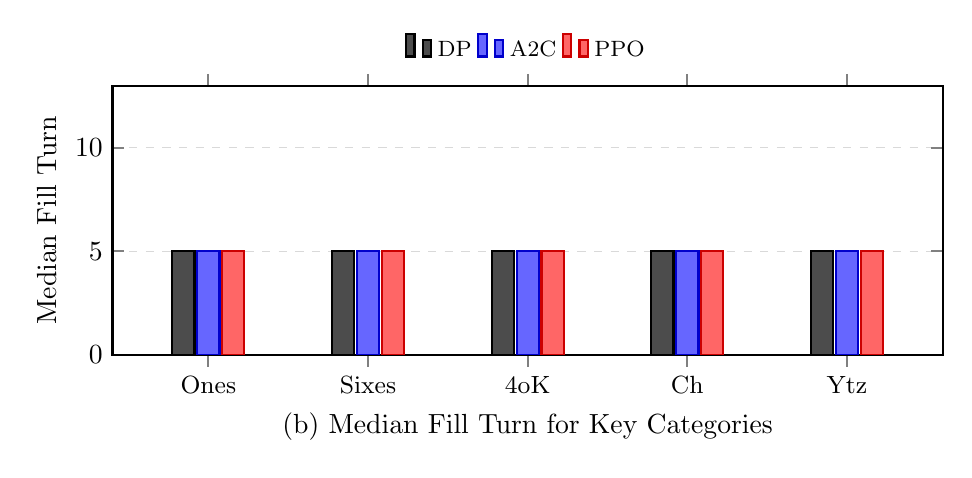
\begin{tikzpicture}
    % Panel (b): Median Fill Turn for Key Categories
    \begin{axis}[
        ybar=1pt,
        width=\columnwidth,
        height=5cm,
        bar width=8pt,
        symbolic x coords={Ones,Sixes,4oK,Ch,Ytz},
        xtick=data,
        xticklabel style={font=\small},
        ylabel={Median Fill Turn},
        xlabel={(b) Median Fill Turn for Key Categories},
        ymin=0,
        ymax=13,
        ymajorgrids=true,
        grid style={dashed,gray!30},
        legend style={
            at={(0.5,1.05)},
            anchor=south,
            legend columns=3,
            font=\footnotesize,
            draw=none,
            fill=none
          },
        enlarge x limits=0.15,
        axis line style={thick},
        tick style={thick},
      ]

      % DP
      \addplot[fill=black!70, draw=black, thick] coordinates {
          (Ones,5) (Sixes,5) (4oK,5) (Ch,5) (Ytz,5)
        };

      % A2C
      \addplot[fill=blue!60, draw=blue!80!black, thick] coordinates {
          (Ones,5) (Sixes,5) (4oK,5) (Ch,5) (Ytz,5)
        };

      % PPO
      \addplot[fill=red!60, draw=red!80!black, thick] coordinates {
          (Ones,5) (Sixes,5) (4oK,5) (Ch,5) (Ytz,5)
        };

      \legend{DP,A2C,PPO}

    \end{axis}
  \end{tikzpicture}
  \caption{Strategy comparison (placeholder data)}
  \label{fig:strategy-comparison}
\end{figure}

<Compare strategies learned by different agents>



\section{Discussion}
% <400-600 words>
\subsection{Summary}
<Discuss implications of results, limitations, and potential improvements.>

\subsection{Strategy \& Failure Modes}
<Analyze common failure modes observed in learned policies>
<Analyze failures during training such as policy collapse>


\section{Conclusion and Future Work}
% <200-300 words>

Learning a robust policy for \textit{Yahtzee} using reinforcement learning presents several interesting challenges and insights.
First, we showed that \textit{Yahtzee}'s combinatorial action space and sparse rewards make it suitable as a non-trivial benchmark environment.
Our results back up theoretical results in the literature regarding training stability and sample efficiency of common RL algorithms.
Likewise, our ablation studies highlight the importance of finding semantically meaningful state and action representations that align the model architecture with the underlying structure of the problem.
Our analysis of learned policies showed that these algorithms often struggle to learn rare, yet high-reward strategies, especially if they require strong coherence over longer time horizons.

Future research could be done to find architectures, samples, and learning methods that allow the model to better approximate optimal play.
For example, curriculum learning approaches, where the agent is gradually exposed to more complex scenarios over time, could be used to help the model overcome some challenges outlined in this paper.

We found that \textrm{Yahtzee} is trivially broken into several a heirarchy of interesting sub-problems.
It was fairly expensive to train a full-game agent from scratch, but training a single-turn agent was much more efficient.
Transfer learning could be explored further to see if knowledge from single-turn optimization could be effectively transferred to full-game, multiplayer Yahtzee, or other variants of the game.
Additionally, \textrm{Yahtzee} could also be considered as a candidate environment for research into hierarchical reinforcement learning (HRL) methods.

Perhaps most interestingly, we showed that an architecture that is, in theory, applicable to the multiplayer setting can be effectively trained to play Solitaire \textit{Yahtzee} at a high level.
This opens the door to future research into adversarial formulations of the game, which are intractable using analytic methods.
Our agent tries only to achieve the best game score, but in a multiplayer setting, it would need to reason about opponents' strategies and scorecards and adapt accordingly to maximize its chances of winning.
Likewise, the use of self-attention and other permutation-invariant architectures could be applicable to many games or scenarios involving multiple agents in a shared environment.

\bibliography{1_introduction,2_related_work,3_methods,4_single_turn_results,5_full_game_experiments,6_discussion,7_appendix}
\bibliographystyle{acl_natbib}

\appendix

\section{Compute Costs}
Experiments were collected using a mix of a local RTX 3090 and AWS-hosted Tesla T4 GPUs.
The total cost of cloud compute was approximately \textbf{\$130}.
Over \textbf{312} training runs were logged in Weights \& Biases, totaling approximately \textbf{566.59 GPU hours}.
The estimated carbon footprint of the compute used is approximately \textbf{A kg CO$_2$e}, based on the methodology from \citet{lacoste-2019-carbontracker}.

\section{AI Usage}

This paper utilized artificial intelligence tools in the following ways:
\begin{itemize}
  \item \textbf{GitHub Copilot (Claude Sonnet 4.5)} was used for typesetting assistance with LaTeX/KaTeX, IDE autocomplete suggestions during coding, and to occassionally perform straightforward refactorings, CUDA performance optimizations, and debugging.
  \item \textbf{ChatGPT (GPT-5.1)} was used for brainstorming ideas for reinforcement learning applications in games, guidance in hyperparameter tuning, helping to outline the structure of this paper, assistance in discovering relevant research and citations, and for writing tone and quality feedback.
\end{itemize}
All other content, including research methodology, analysis, results interpretation, and conclusions, represents original work by the author. The AI tools were not used to generate substantive content or analysis in this document.


\section{Hyperparameters}
The following hyperparameters were used for the baseline models:

\begin{table}[H]
  \centering
  \caption{Shared hyperparameters across all algorithms}
  \label{tab:shared-hyperparameters}
  \begin{tabular}{lc}
    \hline
    \textbf{Hyperparameter}       & \textbf{Value} \\
    \hline
    $d_h$ (Hidden Size)           & 600            \\
    $L$ (Hidden Layers)           & 3              \\
    $p_d$ (Dropout Rate)          & 0.1            \\
    $r_{\alpha}$ (Min LR Ratio)   & 0.01           \\
    $B$ (Games per Batch)         & 20             \\
    Activation Function           & Swish          \\
    Rolling Action Representation & Categorical    \\
    \hline
  \end{tabular}
\end{table}

\begin{table}[H]
  \centering
  \small
  \setlength{\tabcolsep}{4pt}
  \caption{Algorithm-specific hyperparameters}
  \label{tab:algorithm-hyperparameters}
  \begin{tabular}{lccc}
    \hline
    \textbf{Hyperparameter}        & \textbf{REINFORCE} & \textbf{A2C} & \textbf{PPO} \\
    \hline
    $\alpha$                       & 0.001              & 0.0001       & 0.0001       \\
    $\gamma$ (min)                 & 0.95               & 0.99         & 0.99         \\
    $\gamma$ (max)                 & 1.0                & 0.99         & 0.99         \\
    $\tau_{\mathrm{clip}}$         & 0.0                & 1.0          & 1.0          \\
    $\lambda_V$                    & 0.025              & 0.005        & 0.01         \\
    $\beta_{\mathrm{roll}}$ (max)  & 0.1                & 0.06         & 0.02         \\
    $\beta_{\mathrm{roll}}$ (min)  & 0.01               & 0.02         & 0.005        \\
    $\beta_{\mathrm{score}}$ (max) & 0.02               & 0.03         & 0.05         \\
    $\beta_{\mathrm{score}}$ (min) & 0.003              & 0.008        & 0.01         \\
    Entropy Hold Period            & 0.1                & 0.3          & 0.1          \\
    Entropy Anneal Period          & 0.55               & 0.6          & 0.8          \\
    \hline
  \end{tabular}
\end{table}

\begin{table}[H]
  \centering
  \caption{PPO-specific hyperparameters}
  \label{tab:ppo-hyperparameters}
  \begin{tabular}{lc}
    \hline
    \textbf{Hyperparameter} & \textbf{Value} \\
    \hline
    PPO Clip $\epsilon$     & 0.2            \\
    PPO Games per Minibatch & 4              \\
    PPO Epochs              & 3              \\
    \hline
  \end{tabular}
\end{table}

\section{Yahtzee Scoring Rules}
\label{app:scoring}
Next we define the indicator functions for each of the scoring categories:

\begin{align*}
  \mathbb{I}_{3\mathrm{k}}(\mathbf{d})
   & = \mathbb{I}\bigl\{ \max_{v} n_v(\mathbf{d}) \ge 3 \bigr\} \\
  \mathbb{I}_{4\mathrm{k}}(\mathbf{d})
   & = \mathbb{I}\bigl\{ \max_{v} n_v(\mathbf{d}) \ge 4 \bigr\} \\
  \mathbb{I}_{\mathrm{full}}(\mathbf{d})
   & = \mathbb{I}\Bigl\{
  \exists i, j \in \{1, \mathellipsis, 6 \} \ \text{with} \ n_i(\mathbf{d}) = 3 \land n_j(\mathbf{d}) = 2
  \Bigr\}                                                       \\
  \mathbb{I}_{\mathrm{ss}}(\mathbf{d})
   & = \mathbb{I}\Bigl\{
  \exists k \in \{1,2,3\} \ \text{with}\
  \sum_{v=k}^{k+3} \mathbb{I}\{n_v(\mathbf{d}) > 0\} = 4
  \Bigr\}                                                       \\
  \mathbb{I}_{\mathrm{ls}}(\mathbf{d})
   & = \mathbb{I}\Bigl\{
  \exists k \in \{1,2\} \ \text{with}\
  \sum_{v=k}^{k+4} \mathbb{I}\{n_v(\mathbf{d}) > 0\} = 5
  \Bigr\}                                                       \\
  \mathbb{I}_{\mathrm{yahtzee}}(\mathbf{d})
   & = \mathbb{I}\bigl\{\max_v n_v(\mathbf{d}) = 5\bigr\}
\end{align*}

The potential score for each category can then be defined as:
\begin{align*}
  f_j(\mathbf{d})        & = j \cdot n_j(\mathbf{d}), \qquad j \in \{1,\dots,6\}                   \\
  f_7(\mathbf{d})        & = \mathbf{1}^\top \mathbf{d} \cdot \mathbb{I}_{3\mathrm{k}}(\mathbf{d}) \\
  f_8(\mathbf{d})        & = \mathbf{1}^\top \mathbf{d} \cdot \mathbb{I}_{4\mathrm{k}}(\mathbf{d}) \\
  f_9(\mathbf{d})        & = 25 \cdot \mathbb{I}_{\mathrm{full}}(\mathbf{d})                       \\
  f_{10}(\mathbf{d})     & = 30 \cdot \mathbb{I}_{\mathrm{ss}}(\mathbf{d})                         \\
  f_{11}(\mathbf{d})     & = 40 \cdot \mathbb{I}_{\mathrm{ls}}(\mathbf{d})                         \\
  f_{12}(\mathbf{d})     & = 50 \cdot \mathbb{I}_{\mathrm{yahtzee}}(\mathbf{d})                    \\
  f_{13}(\mathbf{d})     & = \mathbf{1}^\top \cdot \mathbf{d}                                      \\
  \mathbf{f}(\mathbf{d}) & =
  \bigl(f_1(\mathbf{d}), f_2(\mathbf{d}), \ldots, f_{13}(\mathbf{d})\bigr)
\end{align*}

\section{State Transition Function}
\label{app:transition-function}

$P$ can be defined by the following generative process.

\begin{itemize}
  \item If $r < 2$ and $a = k$, for each die $i$:
        \begin{itemize}
          \item if $k_i = 1$, keep $d'_i = d_i$;
          \item else sample $d'_i \sim \mathrm{Unif}\{1,\dots,6\}$ independently.
        \end{itemize}
        Set $c' = c,\ r' = r+1,\ t' = t$.
  \item If $r = 2$ and $a = i$, set $d' = d$, update $c' = \mathrm{score}(c,d,i)$,
        set $r' = 0,\ t' = t+1$.
\end{itemize}


\begin{table}[H]
  \centering
  \caption{Category statistics (placeholder data)}
  \label{tab:category-stats}
  \begin{tabular}{lcc}
    \hline
    \multicolumn{1}{c}{\emph{Category}} & $\bar{s}(c)$ & $\sigma^{2}(c)$ \\
    \hline
    Ones                                & $<X>$        & $<Y>$           \\
    Twos                                & $<X>$        & $<Y>$           \\
    Threes                              & $<X>$        & $<Y>$           \\
    Fours                               & $<X>$        & $<Y>$           \\
    Fives                               & $<X>$        & $<Y>$           \\
    Sixes                               & $<X>$        & $<Y>$           \\
    Three of a Kind                     & $<X>$        & $<Y>$           \\
    Four of a Kind                      & $<X>$        & $<Y>$           \\
    Full House                          & $<X>$        & $<Y>$           \\
    Small Straight                      & $<X>$        & $<Y>$           \\
    Large Straight                      & $<X>$        & $<Y>$           \\
    Chance                              & $<X>$        & $<Y>$           \\
    Yahtzee                             & $<X>$        & $<Y>$           \\
    Upper Bonus                         & $<X>$        & $<Y>$           \\
    Yahtzee Bonus                       & $<X>$        & $<Y>$           \\
    \hline
  \end{tabular}
\end{table}



\begin{figure}[H]
  \centering
  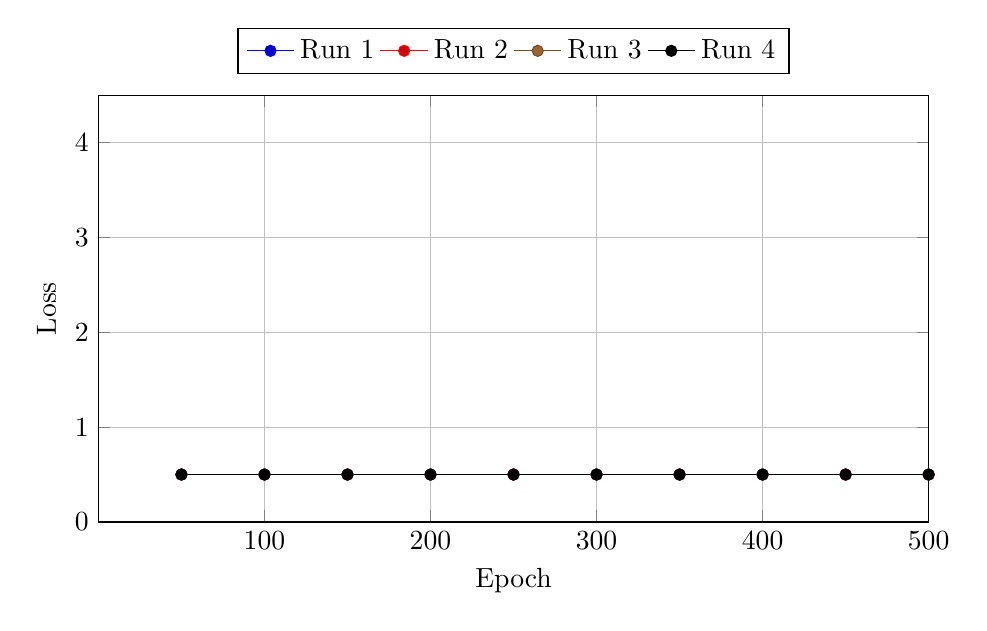
\begin{tikzpicture}
    \begin{axis}[
        width=\columnwidth,
        height=7cm,
        xlabel={Epoch},
        ylabel={Loss},
        xmin=0, xmax=500,
        ymin=0, ymax=4.5,
        xtick={100,200,300,400,500},
        grid=both,
        legend style={at={(0.5,1.05)},anchor=south,legend columns=4},
        mark options={solid},
      ]

      % --- Run 1 (placeholder data around 1) ---
      \addplot+[mark=*] coordinates {
          ( 50,0.5) (100,0.5) (150,0.5) (200,0.5) (250,0.5)
          (300,0.5) (350,0.5) (400,0.5) (450,0.5) (500,0.5)
        };

      % --- Run 2 (placeholder data around 2) ---
      \addplot+[mark=*] coordinates {
          ( 50,0.5) (100,0.5) (150,0.5) (200,0.5) (250,0.5)
          (300,0.5) (350,0.5) (400,0.5) (450,0.5) (500,0.5)
        };

      % --- Run 3 (placeholder data around 3) ---
      \addplot+[mark=*] coordinates {
          ( 50,0.5) (100,0.5) (150,0.5) (200,0.5) (250,0.5)
          (300,0.5) (350,0.5) (400,0.5) (450,0.5) (500,0.5)
        };

      % --- Run 4 (placeholder data around 4) ---
      \addplot+[mark=*] coordinates {
          ( 50,0.5) (100,0.5) (150,0.5) (200,0.5) (250,0.5)
          (300,0.5) (350,0.5) (400,0.5) (450,0.5) (500,0.5)
        };

      \legend{Run 1,Run 2,Run 3,Run 4}

    \end{axis}
  \end{tikzpicture}
  \caption{Training loss (placeholder data)}
  \label{fig:loss-vs-epoch}
\end{figure}

\end{document}
